\documentclass{article}

%----------------------------------------------------------------------------------------
%	REQUIRED PACKAGES and commands
%----------------------------------------------------------------------------------------
\usepackage{amsmath,amsfonts,amssymb,amsthm} % For math equations, theorems, symbols, etc
\usepackage{titlesec} % Allows customization of titles
\usepackage{graphicx}        % Required for including pictures
\usepackage{tikz} % Required for drawing custom shapes
\usepackage{enumitem} % Customize lists
\setlist{nolistsep} % Reduce spacing between bullet points and numbered lists
\usepackage[hidelinks]{hyperref} % make a link between the titles in the table of content and the page of it
\usepackage[a4paper, margin=1in]{geometry}
\usepackage{blindtext}
\usepackage[skip=9pt plus1pt, indent=0pt]{parskip}
\usepackage{wrapfig}
\usepackage{caption2}
\usepackage{flexisym}
\usepackage{comment}
\usepackage[export]{adjustbox}
\usepackage{tcolorbox} % make the enrichment box 
\usepackage{mathrsfs}
\usepackage{siunitx}
\usepackage{eso-pic} % Required for specifying an image background in the title page
\usepackage{mwe}
\usepackage{booktabs} % Required for nicer horizontal rules in tables
\usepackage{lmodern}
\usepackage[T1]{fontenc}
\usepackage{xcolor}
\hyphenpenalty=10000
\definecolor{Solution}{RGB}{0, 135, 189} 
\allowdisplaybreaks
\usetikzlibrary{positioning,calc}
\usetikzlibrary{patterns}
\newcommand*\circled[1]{\tikz[baseline=(char.base)]{
            \node[shape=circle,draw,inner sep=2pt] (char) {#1};}}
\newcommand{\dquad}{\quad\quad}
\newcommand{\tquad}{\quad\quad\quad}
\newcommand{\fquad}{\quad\quad\quad\quad}



%----------------------------------------------------------------------------------------
%	PDF theme color
%----------------------------------------------------------------------------------------

\definecolor{theme}{RGB}{13, 71, 161} % Define the color used for highlighting throughout the pdf

%----------------------------------------------------------------------------------------
%	MAIN TABLE OF CONTENTS
%----------------------------------------------------------------------------------------

\usepackage{titletoc} % Required for manipulating the table of contents

\contentsmargin{0cm} % Removes the default margin

% section text styling
\titlecontents{section}[1.25cm] % Indentation
{\addvspace{5pt}\large\bfseries} % Spacing and font options for sections
{\color{theme!70}\contentslabel[\Large\thecontentslabel]{1.25cm}\color{theme}} % section number
{}  
{\color{theme!70}\normalsize\bfseries\;\titlerule*[.5pc]{.}\;\thecontentspage} % Page number

% Subsection text styling
\titlecontents{subsection}[1.75cm] % Indentation
{\addvspace{1pt}\small} % Spacing and font options for subsections
{\contentslabel[\thecontentslabel]{1.25cm}} % Subsection number
{}
{\;\titlerule*[.5pc]{.}\;\thecontentspage} % Page number
[] 

% Exclude subsubsection from table of contents
\titlecontents{subsubsection}[2cm] % Indentation
{\addvspace{1pt}\small} % Spacing and font options for subsections
{\contentslabel[\thecontentslabel]{1.25cm}} % Subsection number
{}
{\;\titlerule*[.5pc]{.}\;\thecontentspage} % Page number
[]  




\newtheorem{notation}{Notation}[section]

%%%%%%%%%%%%%%%%%%%%%%%%%%%%%%%%%%%%%%%%%%%%%%%%%%%%%%%%%%%%%%%%%%%%%%%%%%%
%%%%%%%%%%%%%%%%%%%% dedicated to boxed/framed environements %%%%%%%%%%%%%%
%%%%%%%%%%%%%%%%%%%%%%%%%%%%%%%%%%%%%%%%%%%%%%%%%%%%%%%%%%%%%%%%%%%%%%%%%%%
\newtheoremstyle{themenumbox}% % Theorem style name
{0pt}% Space above
{0pt}% Space below
{\normalfont}% % Body font
{}% Indent amount
{\small\bf\color{theme}}% % Theorem head font
{\;}% Punctuation after theorem head
{0.25em}% Space after theorem head
{\small\color{theme}\thmname{#1}\nobreakspace\thmnumber{#2}% Theorem text (e.g. Theorem 2.1)
\thmnote{\nobreakspace\textit\bfseries\color{black}---\nobreakspace#3.}} % Optional theorem note
\renewcommand{\qedsymbol}{$\blacksquare$}% Optional qed square

\newtheoremstyle{blacknumex}% Theorem style name
{5pt}% Space above
{5pt}% Space below
{\normalfont}% Body font
{} % Indent amount
{\small\bf}% Theorem head font
{\;}% Punctuation after theorem head
{0.25em}% Space after theorem head
{\small{\tiny\ensuremath{\blacksquare}}\nobreakspace\thmname{#1}\nobreakspace\thmnumber{#2}% Theorem text (e.g. Theorem 2.1)
\thmnote{\nobreakspace\textit\bfseries---\nobreakspace#3.}}% Optional theorem note

\newtheoremstyle{blacknumbox} % Theorem style name
{0pt}% Space above
{0pt}% Space below
{\normalfont}% Body font
{}% Indent amount
{\small\bf}% Theorem head font
{\;}% Punctuation after theorem head
{0.25em}% Space after theorem head
{\small\thmname{#1}\nobreakspace\thmnumber{#2}% Theorem text (e.g. Theorem 2.1)
\thmnote{\nobreakspace\textit\bfseries---\nobreakspace#3.}}% Optional theorem note

%%%%%%%%%%%%%%%%%%%%%%%%%%%%%%%%%%%%%%%%%%%%%%%%%%%%%%%%%%%%%%%%%%%%%%%%%%%
%%%%%%%%%%%%% dedicated to non-boxed/non-framed environements %%%%%%%%%%%%%
%%%%%%%%%%%%%%%%%%%%%%%%%%%%%%%%%%%%%%%%%%%%%%%%%%%%%%%%%%%%%%%%%%%%%%%%%%%
\newtheoremstyle{themenum}% % Theorem style name
{5pt}% Space above
{5pt}% Space below
{\normalfont}% % Body font
{}% Indent amount
{\small\bf\color{theme}}% % Theorem head font
{\;}% Punctuation after theorem head
{0.25em}% Space after theorem head
{\small\color{theme}\thmname{#1}\nobreakspace\thmnumber{#2}% Theorem text (e.g. Theorem 2.1)
\thmnote{\nobreakspace\textit\bfseries\color{black}---\nobreakspace#3.}} % Optional theorem note
\renewcommand{\qedsymbol}{$\blacksquare$}% Optional qed square

\newtheoremstyle{enbox}% % Theorem style name
{0pt}% Space above
{0pt}% Space below
{}
{}
{}
{}
{0.25em}
{\small
\thmnote{\nobreakspace\textit\bfseries\color{black}---\nobreakspace#3.}} % Optional theorem note
\renewcommand{\qedsymbol}{$\blacksquare$}% Optional qed square


\makeatother

\newcounter{dummy}
\numberwithin{dummy}{section}
\theoremstyle{themenumbox}

\newtheorem{theoremeT}[dummy]{Theorem}

\newtheorem{lemma}[dummy]{Lemma}
\newtheorem{observation}[dummy]{Observation}
\newtheorem{proposition}[dummy]{Proposition}
% \newtheorem{definition}[dummy]{Definition}
\newtheorem{claim}[dummy]{Claim}
\newtheorem{fact}[dummy]{Fact}
\newtheorem{assumption}[dummy]{Assumption}

\newtheorem{problem}{Problem}[section]
% \newtheorem{exercise}{Exercise}[section]
\theoremstyle{blacknumex}
\newtheorem{exampleT}{Example}[subsection]
\theoremstyle{blacknumbox}
\newtheorem{vocabulary}{Vocabulary}[section]
\newtheorem{definitionT}{Definition}[section]
\newtheorem{corollaryT}[dummy]{Corollary}




%----------------------------------------------------------------------------------------
%	DEFINITION OF COLORED BOXES
%----------------------------------------------------------------------------------------

\RequirePackage[framemethod=default]{mdframed} % Required for creating the theorem, definition, exercise and corollary boxes

% Theorem box
\newmdenv[
    skipabove=7pt,
    skipbelow=7pt,
    backgroundcolor=black!5,
    linecolor=theme,
    innerleftmargin=5pt,
    innerrightmargin=5pt,
    innertopmargin=5pt,
    leftmargin=0cm,
    rightmargin=0cm,
    innerbottommargin=5pt]{tBox}

% Exercise box	  
\newmdenv[skipabove=7pt,
skipbelow=7pt,
rightline=false,
leftline=true,
topline=false,
bottomline=false,
backgroundcolor=theme!10,
linecolor=theme,
innerleftmargin=5pt,
innerrightmargin=5pt,
innertopmargin=5pt,
innerbottommargin=5pt,
leftmargin=0cm,
rightmargin=0cm,
linewidth=4pt]{eBox}	

% Definition box
\newmdenv[
skipabove=3pt,
skipbelow=3pt,
rightline=false,
leftline=true,
topline=false,
bottomline=false,
linecolor=theme,
innerleftmargin=5pt,
innerrightmargin=5pt,
innertopmargin=0pt,
leftmargin=0cm,
rightmargin=0cm,
linewidth=4pt,
innerbottommargin=0pt]{dBox}	

% Corollary box
\newmdenv[skipabove=7pt,
skipbelow=7pt,
rightline=false,
leftline=true,
topline=false,
bottomline=false,
linecolor=gray,
backgroundcolor=black!5,
innerleftmargin=5pt,
innerrightmargin=5pt,
innertopmargin=5pt,
leftmargin=0cm,
rightmargin=0cm,
linewidth=4pt,
innerbottommargin=5pt]{cBox}

% Creates an environment for each type of theorem and assigns it a theorem text style from the "Theorem Styles" section above and a colored box from above
\newenvironment{theorem}{\begin{tBox}\begin{theoremeT}}{\end{theoremeT}\end{tBox}}
\newenvironment{exercise}{\begin{eBox}\begin{exerciseT}}{\hfill{\color{theme}\tiny\ensuremath{\blacksquare}}\end{exerciseT}\end{eBox}}				  
\newenvironment{definition}{\begin{dBox}\begin{definitionT}}{\end{definitionT}\end{dBox}}	
\newenvironment{example}{\begin{exampleT}}{\hfill{\tiny\ensuremath{\blacksquare}}\end{exampleT}}		
\newenvironment{corollary}{\begin{cBox}\begin{corollaryT}}{\end{corollaryT}\end{cBox}}	
\newenvironment{enrichment*}[1]{\begin{tcolorbox}[colback=theme!5!white,colframe=theme!50!black,title=#1]}{\end{tcolorbox}}



\newenvironment{enrichment}[5]{
    \def\Title{#1}    
    \def\imagepath{#2}
    \def\imagewidth{#3}
    \def\textspace{#4}
    \def\imagespace{#5}
    \begin{tcolorbox}[colback=theme!5!white,colframe=theme!50!black,title=\Title]
        \begin{minipage}[t]{\textspace\textwidth}
        }{
        \end{minipage}
        \hfill
        \begin{minipage}[t]{\imagespace\textwidth}
            \includegraphics[width=\imagewidth cm,valign=t]{\imagepath}
        \end{minipage}
    \end{tcolorbox}
}


%----------------------------------------------------------------------------------------
%	SECTION NUMBERING IN THE MARGIN
%----------------------------------------------------------------------------------------

\makeatletter
\renewcommand{\@seccntformat}[1]{\llap{\textcolor{theme}{\csname the#1\endcsname}\hspace{1em}}}                    
\renewcommand{\section}{\@startsection{section}{1}{\z@}
{-4ex \@plus -1ex \@minus -.4ex}
{1ex \@plus.2ex }
{\normalfont\large\bfseries}}
\renewcommand{\subsection}{\@startsection {subsection}{2}{\z@}
{-3ex \@plus -0.1ex \@minus -.4ex}
{0.5ex \@plus.2ex }
{\normalfont\bfseries}}
\renewcommand{\subsubsection}{\@startsection {subsubsection}{3}{\z@}
{-2ex \@plus -0.1ex \@minus -.2ex}
{.2ex \@plus.2ex }
{\normalfont\small\bfseries}}                        
\renewcommand\paragraph{\@startsection{paragraph}{4}{\z@}
{-2ex \@plus-.2ex \@minus .2ex}
{.1ex}
{\normalfont\small\bfseries}}






\definecolor{c1}{RGB}{100, 0, 0}

\definecolor{c2}{RGB}{0, 100, 0}


\newenvironment{Framesofreference}{
    \begin{center}
        \begin{tikzpicture}
            \draw[->] (0,0,0) -- (8,0,0) node[right]{$x$};
            \draw[->] (0,0,0) -- (0,3,0) node[above]{$y$};
            \draw[->] (0,0,0) -- (0,0,3) node[below left]{$z$};    
            \draw (0,0,0) node[below right] {$O$};
            \draw (2,2.7,0) node{$S$};
            \draw[-> , blue] (4,0,0) -- (9,0,0) node[right]{$x'$};
            \draw[-> , blue] (4,0,0) -- (4,3,0) node[above]{$y'$};
            \draw[-> , blue] (4,0,0) -- (4,0,3) node[below left]{$z'$};
            \draw[dashed,->] (4,1.5,0) -- (5,1.5,0) node[above]{$v$};
            \draw[blue] (4,0,0) node[below right] {$O'$};
            \draw (6,2.7,0) node{$S'$};
}{
\end{tikzpicture}\end{center}
}


\begin{document}


%----------------------------------------------------------------------------------------
%	TITLE PAGE
%----------------------------------------------------------------------------------------
\begingroup
\pagenumbering{gobble}
\AddToShipoutPicture*{\put(0,0){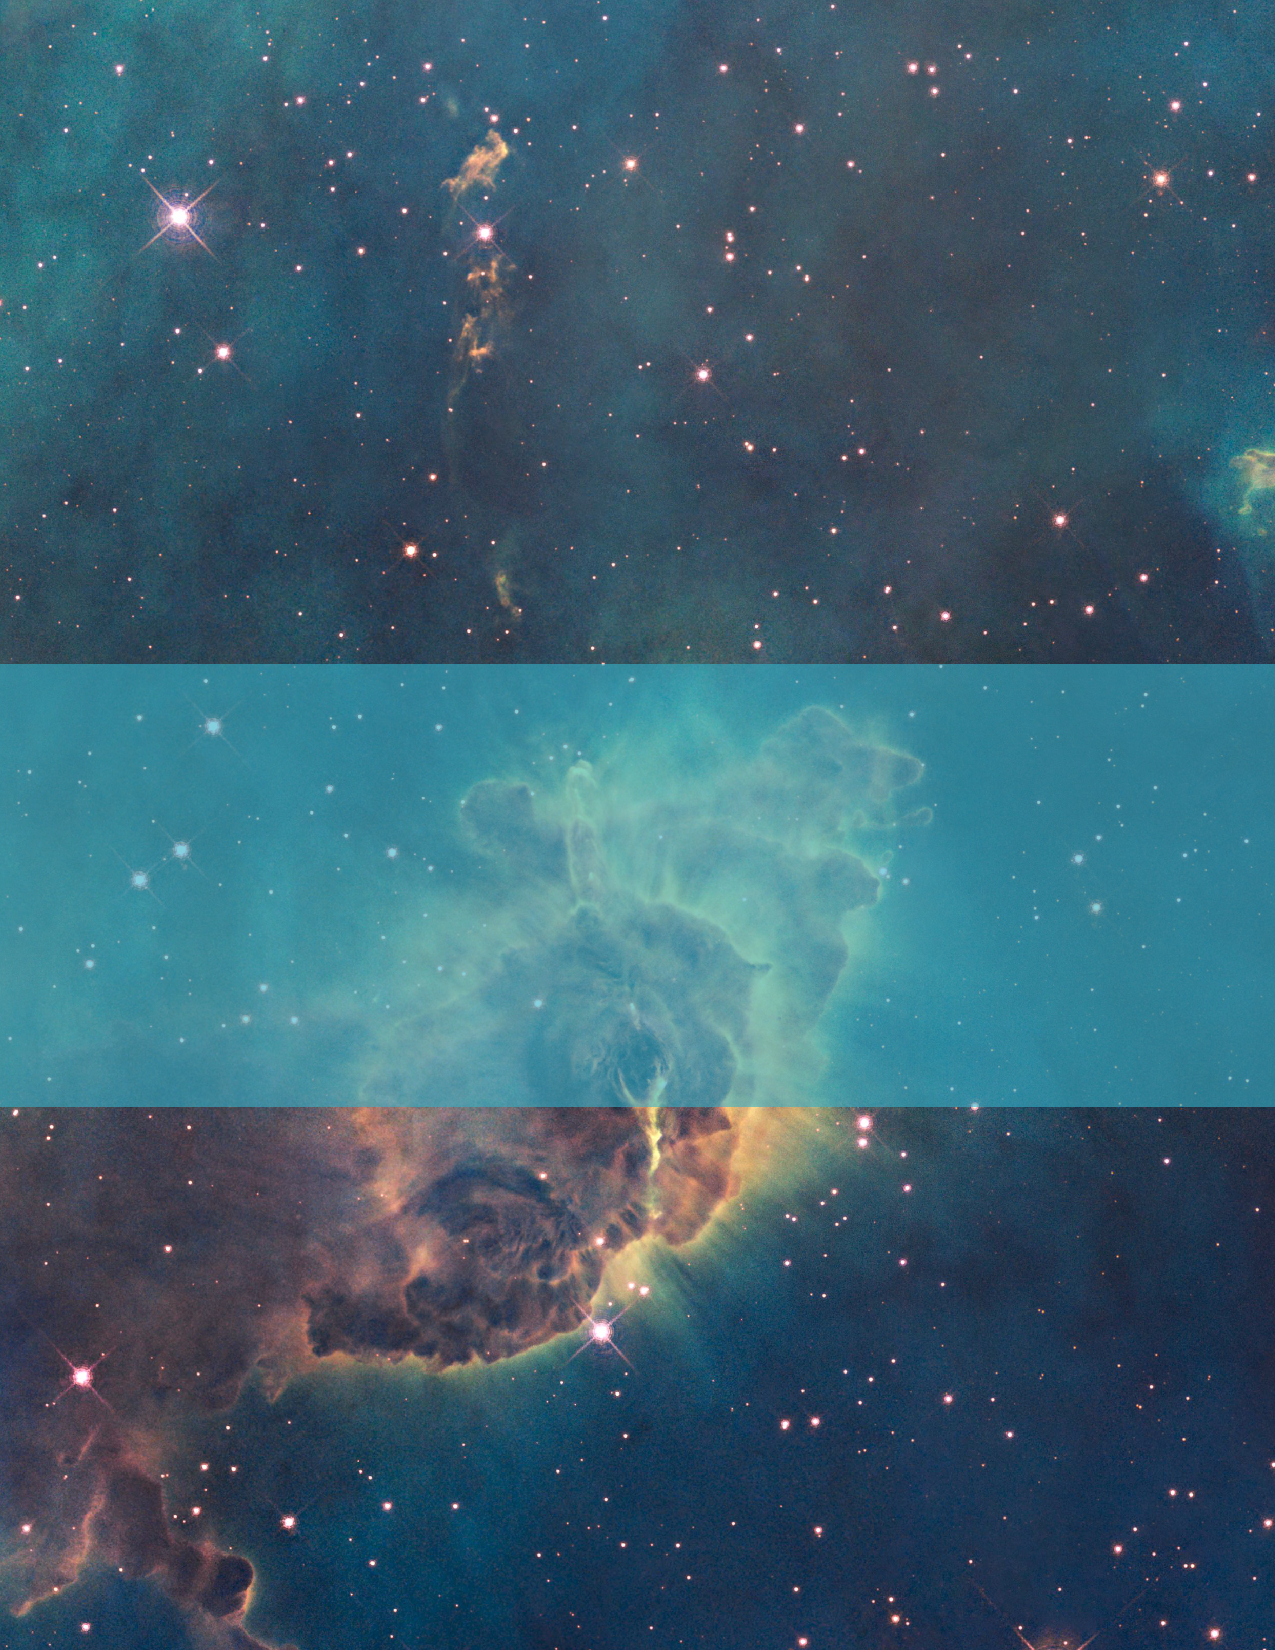
\includegraphics[scale=1.25]{Cover}}}
\centering
\vspace*{6cm}
\par\normalfont\fontsize{30}{30}\sffamily\selectfont
\textbf{Theory Of Special Relativity}\\
{\LARGE 01356 Spring 2023}\par
\vspace*{1cm}
{\Huge Lecture Notes}\par
\vspace*{1cm}
{\Huge Lecturer: Prof.Kamal Mostafa}\par
{\Huge Prepared by: Ahmed.M.Habib}\par
\endgroup


\newpage
\pagenumbering{arabic}

\tableofcontents 



\newpage

%\sectionimage{head1.png}
\section{Introduction}
The theory of relativity, introduced by Albert Einstein in the early 20th century, revolutionized our understanding of space, time, and gravity. It consists of two major branches: special relativity and general relativity. While both theories share the common foundation of relativity, they address different aspects of the physical world and have distinct principles and applications.


\subsection{Special Relativity}
Special relativity, formulated by Einstein in 1905, deals with the behavior of objects moving at constant speeds, particularly in the absence of gravitational fields. It is based on two postulates: the principle of relativity and the constancy of the speed of light.\par
The principle of relativity states that the laws of physics are the same for all observers in uniform motion. This means that there is no preferred reference frame, and the fundamental laws of nature should be invariant under certain transformations. It introduced the concept of time dilation, where time appears to move slower for an object in motion relative to a stationary observer.\par
The constancy of the speed of light postulate asserts that the speed of light in a vacuum is always the same, regardless of the motion of the source or the observer. This leads to the phenomenon of length contraction, where objects moving at high speeds appear shorter along their direction of motion.\par

\subsection{General Relativity}

\begin{wrapfigure}{r}{0.4\textwidth}
    \centering
    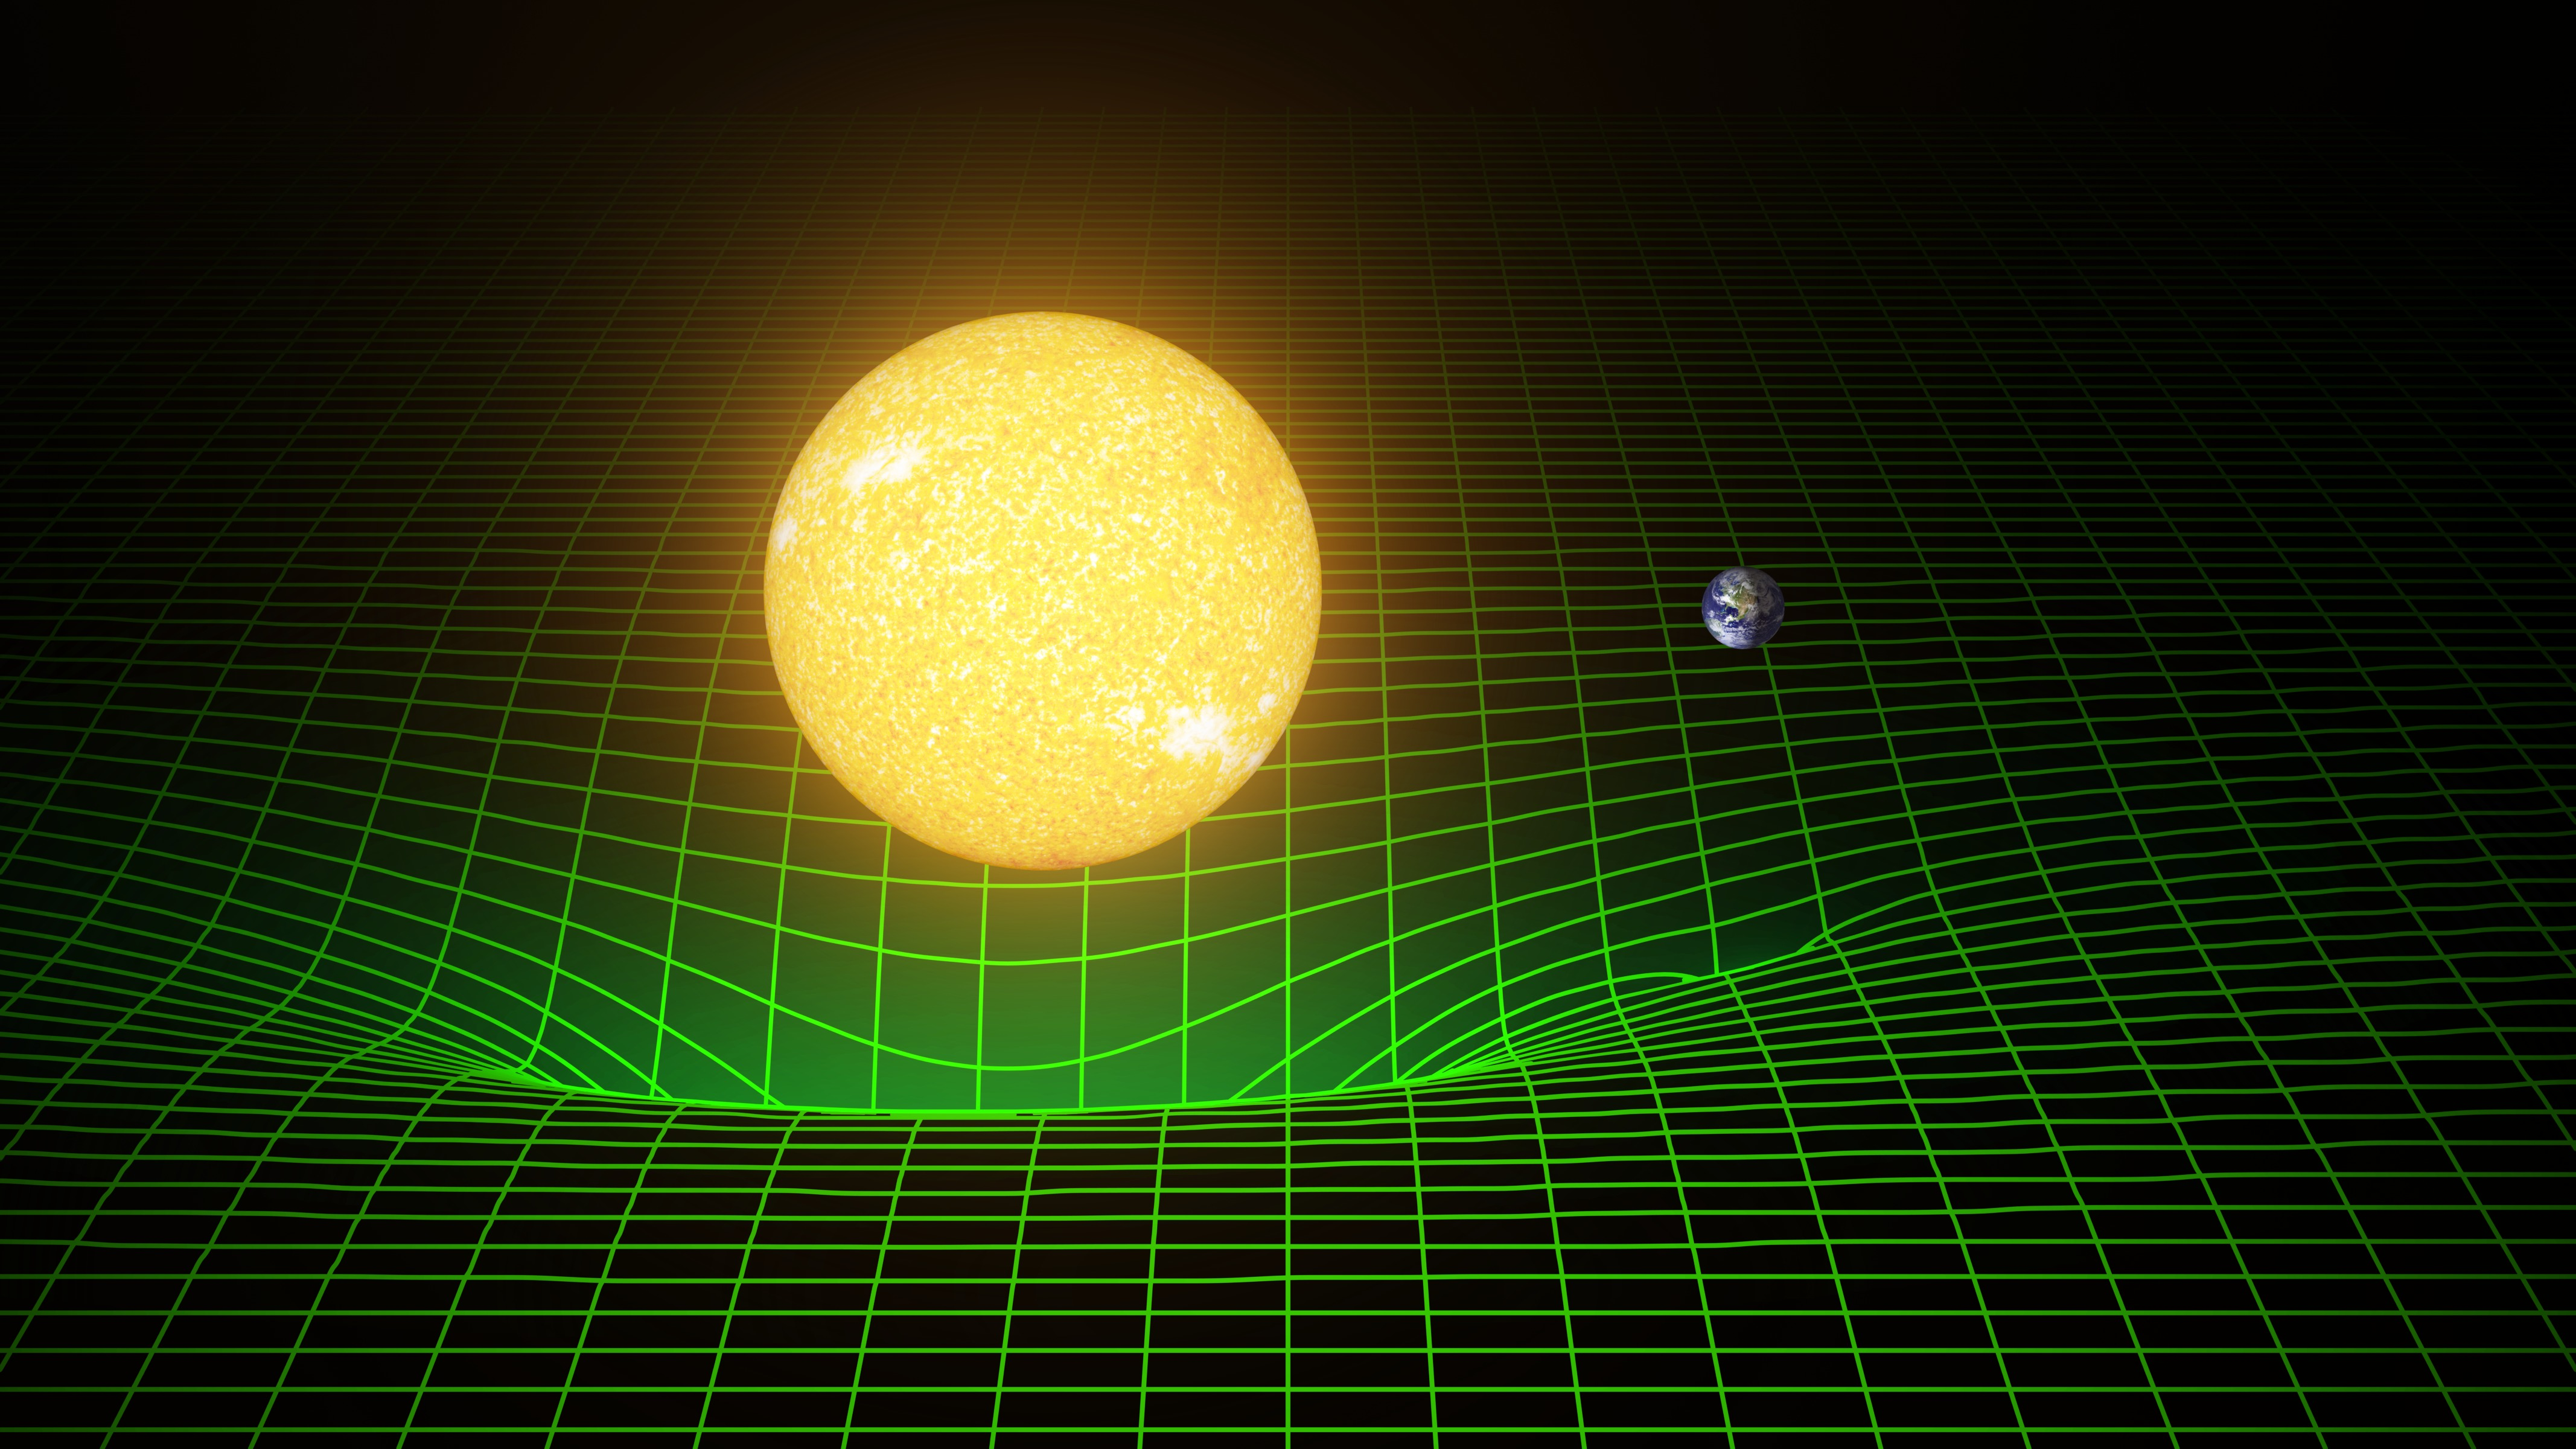
\includegraphics[width=1\linewidth,keepaspectratio]{spacetimefabric}
    \captionlabelfalse
    \caption{spacetime fabric}
    \label{fig:spacetimefabric} 
\end{wrapfigure}
General relativity, published by Einstein in 1915, extends the principles of special relativity to include gravitational effects and the curvature of spacetime. It describes gravity as the curvature of spacetime caused by the presence of mass and energy as shown in the figure.\par
According to general relativity, mass and energy curve the fabric of spacetime, creating what we perceive as gravity. Objects move along the curved paths dictated by this geometry. The theory provides a more comprehensive understanding of gravity and predicts phenomena such as gravitational time dilation, gravitational waves, and the bending of light by massive objects.\par
General relativity also led to the concept of black holes, which are regions of spacetime where the gravitational field is so strong that nothing, not even light, can escape. It has been confirmed by numerous experiments and observations, including the bending of starlight during a solar eclipse and the detection of gravitational waves.\par

\subsection{Summary}
The subject of our study in this course will be only the Special Relativity. 

So to summarize the above
The Special Relativity deals with systems moving with uniform velocity
The postulates of the Special Relativity is
\begin{enumerate}
\item the speed of light in a vacuum is always the same, regardless of the motion of the source or the observer. 
\item the natural laws must preserve their forms relative to all observers in a state of relative uniform motion.
\end{enumerate}

\newpage
\section{Galilean Transformation}
Consider the two frames $S$ and $S'$ of references one at rest and one moving with uniform velocity $V$\\
Let $O$ and $O'$ be the observers situated at the origins of $S$ and $S'$ respectively.\\
They are observing the same event at any point $p$.\\
Let the two frames be parallel to each other as shown in the Figure
\begin{Framesofreference}
\end{Framesofreference}
The origins of the two frames is chosen such that they coincide at time $t$ and $t'$\\
Galileo considered the time is absolute i.e. $t = t'$.
 also he considered the mass and the force are also absolute i.e. $m = m'$ and $F = F'$.\\
Therefore
\begin{equation}
    \label{eq:GT}
    \begin{cases}
    &x' = x-vt\\
    &y' =y\\
    &z' =z\\
    &t' =t
\end{cases}    
\end{equation}
equations (\ref{eq:GT}) is called the Galilean Transformation and it preserve the form of the natural laws as newton's second law as follows:
\begin{align*}
    \because F &= m\frac{d^2x}{dt^2}\\
    \because  \frac{dx'}{dt'} &= \frac{dx'}{dt} = \frac{dx}{dt} - v\\ 
    \therefore \frac{d^2x'}{d{t'}^2} &= \frac{d^2x}{dt^2}\\
    \therefore m'\frac{d^2x'}{d{t'}^2} &= m'\frac{d^2x}{dt^2} = m\frac{d^2x}{dt^2}\\
    \therefore F' &= F
\end{align*}

\begin{figure*}[b]
    \begin{enrichment}{Galileo Galilei}{galilio.jpg}{2.4}{.8}{.17}
        born in 1564, Galileo Galilei was an Italian astronomer, mathematician, and physicist who made significant contributions to the scientific revolution. 
        Known as the "father of modern science," Galileo played a crucial role in advancing our understanding of the natural world. 
        He is famous for his observations using the telescope, which he built and improved upon.
    \end{enrichment}
\end{figure*}

\newpage

\section{Lorentz Transformation And it's consequences}
\subsection{Lorentz Transformation(L.T)}
Lorentz Transformation can be derived on the basis of the two postulates or principles.
\begin{itemize}
    \item laws of physics are the same form in all frames
    \item  the speed of light is constant in all frames 
\end{itemize}
Consider the two frames $S$ and $S'$ as mentioned before

\begin{Framesofreference}
    \draw[<-] (0,2,0) -- (1.75,2,0) node[right]{$vt$};
    \draw[->] (2.25,2,0) -- (4,2,0) node[right]{};

    \fill[draw=black, fill=red] (6.7,1,1) circle[radius=2pt];
    \node[below right] at (6.7,1.2,1) {$p$};
    \node[below right] at (6.9,1.5,1) {$(x,y,z,t)$};
    \node[below right] at (6.9,1.1,1) {$(x',y',z',t')$};
\end{Framesofreference}

let the observers in the two frames be situated at the origins $O$ and $O'$ the are observing the same event at the point $p$ whose coordinates are $(x,y,z,t)$ and $(x',y',z',t')$ in $S$ and $S'$ respectively.\\
points at rest relative to $S'$ will move with velocity $V$ relative to $S$.\\
\subsubsection{Lorentz Factor}
in particular the point $x' = 0$ will move with velocity $V$ in $x-$direction will be identical with $x=vt$ , so that 
\setcounter{equation}{0}
\begin{equation}
    x' = \beta(x-vt)
    \ \ , \ \
    y' = y 
    \ \ , \ \
    z' = z
\end{equation}
now we have to formulate an equation in $t$ and $t'$ where $t'$ depends on $x,y,z,t$ linearly so 
\begin{equation}
    t' = \alpha t + \gamma x
\end{equation}
where $\alpha , \beta , \gamma$ are functions in $v$ only , we going to determine the unknowns $\alpha , \beta , \gamma$\\
Let us assume that at time $t=0$ a spherical wave of light signal leaves $O$ which coincides with $O'$ at the same moment\\
it progress in therefore described by 
\begin{equation}
    x^2+y^2+z^2=c^2t^2
\end{equation}
and
\begin{equation}
    {x'}^2+{y'}^2+{z'}^2=c^2{t'}^2
\end{equation}
using equations (1) and (2) and substitute in (4)
we get the following
\begin{equation}
    \label{eq:5.1}
    \beta^2{(x-vt)}^2+y^2+z^2=c^2{(\alpha t + \gamma x)}^2
\end{equation}
this equation and equation (3) represent the same motion, so 
\begin{equation}
    \beta^2-c^2\gamma^2 = 1 \ \ \ (\text{coefficient of }x^2)
\end{equation}

\begin{equation}
    \beta^2 v +c^2\alpha\gamma = 0 \ \ \ (\text{coefficient of }xt)
\end{equation}

\begin{equation}
    c^2\alpha^2 - \beta^2 v^2  = c^2   \ \ \ (\text{coefficient of }t^2)
\end{equation}

by eliminate $\beta$ from (6) and (7)
\[
    \hspace{-3.5cm}
    v\times(6) - (7) \Longrightarrow
    \hspace{1cm}
    -c^2\gamma^2 v - c^2\alpha\gamma = v
\]
\begin{equation}
    \therefore \  v(1+c^2\gamma^2) + c^2\alpha\gamma = 0
\end{equation}
also
\[
    \hspace{-3.5cm}
    v^2 \times(6) + (8) \Longrightarrow  
    \hspace{1cm}
    -c^2\gamma^2 v^2 + c^2\gamma^2 = v^2+c^2
\]
\begin{equation}
    \therefore \  -v^2(1+c^2\gamma^2) + c^2\alpha^2 = c^2
\end{equation}
then
\begin{align*}
    \hspace{-3.5cm}
    v\times(9) + (10) \Longrightarrow 
    \hspace{1cm} 
    v c^2\gamma\alpha + c^2\alpha^2 &= c^2\\
    \therefore  \ v\gamma\alpha + \alpha^2 &= 1
\end{align*}
\begin{equation}
    \therefore \  \alpha^2 - 1 = -v\gamma\alpha
\end{equation}
the equations (9) and (11) are two equations on $\alpha$ and $\gamma$ by eliminating $\gamma$ we get
\begin{align*}
    v \left\{1+ c^2{\left[\frac{(\alpha^2 -1)}{-v \alpha} \right]}^2\right\} + \frac{c^2(\alpha^2 -1)\alpha}{-v \alpha} &= 0\\
    v \left\{\frac{v^2 \alpha^2 +c^2{(\alpha^2 -1)}^2}{v^2 \alpha^2}\right\} + \frac{c^2(\alpha^2 -1)}{-v} &= 0\\
    \therefore  \ v^2 \alpha^2 + c^2{(\alpha^2 -1)}^2 - \alpha^2 c^2(\alpha^2 -1) &=0\\
    \alpha^2(c^2-v^2)=c^2    \ \ \ \ \ \ \   \therefore  \alpha^2 = \frac{c^2}{c^2-v^2} &
\end{align*}
using equation (8)
\begin{align*}
    \therefore  c^2 &\left(\frac{c^2}{c^2-v^2}\right) - \beta^2 v^2 = c^2 \\
    \beta^2 &= \frac{c^2}{c^2-v^2} = \alpha^2\\
    \therefore   \beta &= \alpha = \frac{1}{\sqrt{1-\frac{v^2}{c^2}}} 
\end{align*}
using the equation (7)
\[
    \left(\frac{1}{1-\frac{v^2}{c^2}}\right) v + \gamma c^2 \frac{1}{\sqrt{1-\frac{v^2}{c^2}}} = 0
\]
\[
\therefore \ \frac{v}{\sqrt{1-\frac{v^2}{c^2}}} = -c^2 \gamma
\]
\[
\therefore \ \gamma = \frac{-v \beta}{c^2}
\]
from (2)
\[
t' = \alpha t + \gamma x = \beta t + \frac{-v \beta x}{c^2}
\]
\[
\therefore \ t' = \beta\left(t - \frac{vx}{c^2}\right)
\]
\setcounter{equation}{1}
so we have
\begin{equation}
    \begin{cases}
    &x' = \beta(x-vt)\\
    &y' =y\\
    &z' =z\\
    &t' =\beta\left(t - \frac{vx}{c^2}\right)
    \end{cases}    
\end{equation}
the equations (2) are called Lorentz Transformation where $\beta = \frac{1}{\sqrt{1-\frac{v^2}{c^2}}}$.
\begin{observation}
    if v is very small compare to c $ \ \ \ \therefore \frac{v}{c} \to 0$ so the $\beta \to 1$\\
    in that case Lorentz transformation becomes 
    \[
        x' = x-vt  \ \ ,
        y' =y   \ \ ,
        z' =z   \ \ ,
        t' =t
    \]
    those are the Galilean Transformation\\
    thus Lorentz Transformation reduce to Galilean Transformation if $v \ll c$
\end{observation}



\subsection{Lorentz Inverse Transformation(L.I.T)}
here we will do the opposite of what we did in L.T instead of getting $x,y,z,t$ in terms of $x' , y' , z' , t'$
now we will get $x' , y' , z' , t'$ in terms of $x,y,z,t$ 

\begin{align*}
    \because x' &= \beta(x-vt)\\
    \therefore x &= \frac{x'}{\beta} + v\left(\frac{t'}{\beta} + \frac{vx}{c^2}\right)\\
    x\left(1-\frac{v^2}{c^2}\right) &= \frac{x'}{\beta} + \frac{vt'}{\beta}    \\
    \because \beta &= \frac{1}{\sqrt{1-\frac{v^2}{c^2}}}\\
    \therefore \frac{x}{\beta^2} &= \frac{x'}{\beta} + \frac{vt'}{\beta}    \\
    \therefore x &= \beta(x'+vt')
\end{align*}
in the same manner we can get that 
\[
\therefore t =\beta\left(t' + \frac{vx'}{c^2}\right)
\]
so we have 
\[
        x= \beta(x'+vt')
        \ \ , \ \ 
        y = y'
        \ \ , \ \ 
        z = z'
        \ \ , \ \
        t =\beta\left(t' + \frac{vx'}{c^2}\right)
\]
those equations is called Lorentz inverse transformation
we notice that we can obtain L.I.T from L.T by replacing $v$ with $-v$
which make sense actually because it's like saying that the observer instead of standing on the frame at rest he stand on the moving frame whose velocity $v$ in the $x$-direction he then will Consider himself at rest and the frame that in rest he will see it moving in velocity $-v$ in $x$-direction
\begin{figure*}[b]
    \begin{enrichment}{Hendrik Lorentz}{Lorentz.jpg}{2.4}{.8}{.17}
    born in 1853 Hendrik Lorentz was a Dutch physicist who made significant contributions to the field of theoretical physics.
    He is best known for his work on electromagnetic theory and his formulation of the Lorentz transformation, which played a fundamental role in the development of Albert Einstein's theory of relativity. 
    Lorentz's research focused on the behavior of electrically charged particles and their interaction with electromagnetic fields. 
    His theories laid the foundation for understanding phenomena such as the Lorentz force and the behavior of light in moving media.
    \end{enrichment}
\end{figure*}

\pagebreak 
\subsection{Length Contraction}
now we will discuss some consequences of Lorentz Transformation \\
suppose that a rod is at rest on $x'$-axis in the frame $S'$ and so also the rod is moving with velocity $v$ along $x$-axis with respect to the frame $S$

\begin{Framesofreference}
    \fill[color=c2] (5,0,0) circle[radius=1.5pt];
        \fill[color=c2] (6,0,0) circle[radius=1.5pt,];

        \draw[line width=3pt , color=c2] (5,0) -- (6,0);
        \node[above, color=c1] at (5,0,0) {$x_1$};
        \node[above, color=c1] at (6,0,0) {$x_2$};
        \node[below, color=c1] at (5,0,0) {$x'_1$};
        \node[below, color=c1] at (6,0,0) {$x'_2$};
\end{Framesofreference}
let the two ends of the rod be labeled $x_1$,$x_2$ in $S$ and $x'_1$,$x'_2$ in $S'$\\
then $x'_2-x'_1=L_o'$ is the length of the rod in the frame $S'$ in which it is at rest by Lorentz Transformation
\[
L_o' = x'_2-x'_1 = \beta(x_2-vt_2) - \beta(x_1-vt_1)
\]
where $t_2$ and $t_1$ are the times at which the observer in $S$ measures the end points
\[
L_o' = \beta(x_2-x_1) - \beta v(t_2-t_1)
\]
now to measure the length $L = x_2-x_1$ in the frame $S$, it is necessary that the end points $x_1$ and $x_2$ are measured simultaneously in $S$ i.e. $t_1=t_2$
\[
\therefore L_o' = \beta(x_2-x_1) = \beta L
\]
and since $\beta = \frac{1}{\sqrt{1-\frac{v^2}{c^2}}} > 1$
\[
\therefore L_o' > L
\]
This means that the observer in $S$ see the moving rod shorter as compared to it's original length
\begin{enumerate}
    \item the shortening of length for moving object is called length contraction or space contraction or Lorentz contraction
    \item proper length : the proper length of an object is defined as it's length measured in a reference frame in which the object is at rest 
\end{enumerate}
\pagebreak
\subsection{Time Dilation}
consider two frames $S$ and $S'$ as shown 

\begin{Framesofreference}
    \draw[|-] (4,.2,0) -- (4.27,.2,0);
    \draw (4.5,.25,0) node{$x'$};
    \draw[-|] (4.7,.2,0) -- (5,.2,0);
    \fill[color=red] (5.1,0,0) circle[radius=2pt];
\end{Framesofreference}

suppose a clock at rest at $(x',0,0)$ in $S'$ 
sends one light flash at time $t'_1$\\
and the next one at time $t'_2$ in $S'$. the time between the two events (the two flashes) is 
\[
\Delta T_o' = t'_2 - t'_1
\]
the corresponding times as observed by an observer in $S$ on his clock are respectively
\[
t_1 = \beta\left(t'_1 + \frac{vx'}{c^2}\right) \ \ \ \ and  \ \ \ \ t_2 = \beta\left(t'_2 + \frac{vx'}{c^2}\right)
\]
hence the time interval between the two events as measured in $S$ is 
\[
\Delta T = t_2-t_1 = \beta (t'_2-t'_1) = \beta\Delta T_o' \ \ \ \ \ \ \ ,\beta>1
\]
\[
\therefore \Delta T > \Delta T_o'
\]
i.e. Time interval as recorded by the observer in $S$ between the two moving event in $S'$ is longer than the time interval recorded by the observer in the $S'$
on a clock which is at rest with respect to where the event occur \\
this relativistic effect is called time dilation

\subsection{Simultaneity}
\hfill
\begin{definition}
    Two event are said to be simultaneous if they occur at the same time.    
\end{definition}
\begin{theorem}
    Simultaneity has only a relative and not an absolute meaning
\end{theorem}
\begin{proof}
consider two frames $S$ and $S'$, where $S'$ is moving with uniform velocity $v$ along $x$-axis\\
let two events occur simultaneously in $S$ at two different points $P_1(x_1,y_1,z_1,t_1)$ and $P_2(x_2,y_2,z_2,t_2)$
such that $x_1 \neq x_2 $.\\
$\because$ the events are simultaneous in $S \ \ \ \ \therefore t_1=t_2$\\
let $t'_1$ and $t'_2$ be the time in $S'$ corresponding to the times $t_1$ and $t_2$ in $S$ by Lorentz Transformation we have 
\[
    t'_1 = \beta\left(t_1 - \frac{vx_1}{c^2}\right) \ \ \ \ \text{and}  \ \ \ \ t'_2 = \beta\left(t_2 - \frac{vx_2}{c^2}\right)
\]
\[
t'_2 -t'_1 = \beta(t_2-t_1) + \frac{\beta v}{c^2}(x_1-x_2) \ \ \ ,\because t_1=t_2
\]
\[
\therefore t'_2 -t'_1 = \frac{\beta v}{c^2}(x_1-x_2) \ \ \ ,\because x_1 \neq x_2
\]
\[
\therefore t'_2 -t'_1 \neq 0  \ \ \ ,\therefore t_1 \neq t_2
\]
\end{proof}
this means that the same two events are not simultaneous in $S'$\\
i.e. Two events at different places which are simultaneous for an observer at rest in $S$ , are no longer simultaneous to an observer $S'$ which is moving with velocity $v$ relative to $S$ along $x$-axis

\subsection{Examples}
\begin{example}
    Imagine that a 40 years old scientist falls in love with 18 years old girl who is his laboratory assistant.
    they want to marry but they feel that their marriage can not be welcomed by the society due to the age difference.
    scientist plans to marry using the principle of time dilation of relativity. so he synchronizes his clock with that of his assistant and goes to a long journey in a rocket with velocity 0.999c\\
    he returns back when his clock pass one year but he find in her clock 22.7 years have passed 
    \[
    \Delta T = \beta\Delta T'_o = \frac{1}{\sqrt{1-\frac{{(0.999c)}^2}{c^2}}} \times 1 = 22.7\si{years}
    \]
    now the scientist is 40+1 = 41 years and his assistant is 18+22.7 = 40.7 years old their age difference barrier has now been overcome therefore they marry    
\end{example}
\begin{example}
    what is the velocity of a rod if it's length is observed to be $0.99L'_o$? where $L'_o$ is it's proper length
\begin{center}
    ------ \textcolor{Solution}{Solution} ------ 
\end{center}
\[
\because L'_o = \beta L \ \ \ \ \ \ \ \therefore L'_o = \beta(0.99L'_o)
\]
\[
\sqrt{1-\frac{v^2}{c^2}} = 0.99 \ \ \ \ \ \ \ \therefore \frac{v^2}{c^2} = 1-0.99^2
\]
\[
\therefore v = 0.141c
\]
\end{example}
\begin{example}
    two light pulses are moving in the positive direction of $x$-axis of the frame $S$. the distance between them being $d$. what is their distance of separation as seen from frame $S'$ moving with velocity $v$ along the positive direction of $x$-axis with respect to $S$
    \begin{center}
        ------ \textcolor{Solution}{Solution} ------
    \end{center}
    suppose one pulse passes the origin $O$ at time $t=0$ in $S$\\
    it's equation of motion is 
    \setcounter{equation}{0}
    \begin{equation}
        x_1=ct
    \end{equation}
    the other pulse has the equation
    \begin{equation}
        x_2=ct+d
    \end{equation}
    in the frame $S'$
    \begin{equation}
    \circled{1}  \Longrightarrow  \ \ \ \ \ \ \beta(x'_1+vt') = c\beta\left(t'+\frac{vx'_1}{c^2}\right)
    \end{equation}
    \begin{equation}
        \circled{2}  \Longrightarrow  \ \ \ \ \ \ \beta(x'_2+vt') = c\beta\left(t'+\frac{vx'_2}{c^2}\right) + d
    \end{equation}
    we have to find $x'_2-x'_1$\\
    by subtract $(4)-(3)$ we get
    \[
    \beta(x'_2-x'_1)=\frac{c\beta v}{c^2}(x'_2-x'_1) + d
    \]
    \[
    (x'_2-x'_1)(1-\frac{v}{c})=\frac{d}{\beta} \ \ \ \ \ \therefore x'_2-x'_1 = \frac{\sqrt{1-\frac{v^2}{c^2}} \times d}{1-\frac{v}{c}}
    \]
    \[
    \therefore x'_2-x'_1 = \sqrt{\frac{c+v}{c-v}} \times d
    \]
\end{example}
\begin{example}
    at what speed should a clock be moving so that it may appear to lose 1 minute in each hour
\begin{center}
    ------ \textcolor{Solution}{Solution} ------
\end{center}
    since the clock is to loose one minute in each hour ,hence the moving clock records 59 minute for each hour recorded by clock stationary relative to the observer.\\
    \[
    \Delta T'_o = 59\text{ minute \ \ \ \ and\ \ }\Delta T=60 \si{min}
    \]
    \[
    \because \Delta T = \beta\Delta T'_o 
    \]
    \[
    60 = \frac{1}{\sqrt{1-\frac{v^2}{c^2}}}(59) \ \ \Longrightarrow \ \  1-\frac{v^2}{c^2} = {\left(\frac{59}{60}\right)}^2
    \]
    \[
    \frac{v^2}{c^2} = \frac{119}{60^2} \ \ \Longrightarrow \ \ v=\frac{\sqrt{119}}{60}c
    \]
\end{example}
\begin{example}
    a body has the dimension represented by $6 \hat{i}+7 \hat{j}$ meters in reference system $S'$.how those dimension will be represented in the system $S$ if $S'$ is moving with velocity $0.6c$
    
    \begin{center}
        ------ \textcolor{Solution}{Solution} ------
    \end{center}
    \begin{Framesofreference}
        \draw[|-] (5.5,-.2,0) -- (6.3,-.2,0);
        \draw (6.5,-.25,0) node{$6$};
        \draw[-|] (6.7,-.2,0) -- (7.5,-.2,0);
        
        \draw[-|] (7.7,1.4,0) -- (7.7,2.33,0);
        \draw (7.7,1.16,0) node{$7$};
        \draw[-] (7.7,0,0) -- (7.7,.9,0);

        \foreach \y in {-4,-3,-2,-1,0,1,2,3,4}
        \draw[red,pattern=north east lines,pattern color=gray] (5.5,0) -- (5.5,2.33)--(7.5,2.33) -- (7.5,0);
    \end{Framesofreference}  
    by Lorentz transformation
\[
    L'_0 = \beta L
\]
\[
    L = L'_0 \sqrt{1-\frac{v^2}{c^2}} \ \ \ \ \ , v=0.6c
\]
the contraction will be only for the length in $x$-direction
\[
    \therefore L_x = 6\sqrt{1-0.36} = 6\times0.8 = 4.8 \si{m}
\]
i.e. the dimensions of the body in the system $S$ is $4.8 \hat{i}+7 \hat{j}$ there is no contraction in the direction of $y$-axis , since there is no motion along $y$-axis in $S'$  
\end{example}
\newpage
\begin{example}
    the length of a rocket ship is 100 meters on the ground when it fly the observer on the ground sees it 99 meters. calculate it's speed
    \begin{center}
        ------ \textcolor{Solution}{Solution} ------
    \end{center}
    \begin{align*}
        L'_o &= \beta L    \\
        L &= L'_o \sqrt{1-\frac{v^2}{c^2}}    \\
        99 &= 100 \sqrt{1-\frac{v^2}{c^2}} \\ 
        v &= \frac{\sqrt{199}}{100}c 
    \end{align*}
\end{example}

\begin{example}
    calculate the length of a rod moving with velocity 0.8c in a direction inclined at $60^\circ$ to it's own length the proper length of the rod is given by 100cm
    
    \begin{center}
        ------ \textcolor{Solution}{Solution} ------
    \end{center}

    \begin{center}
        \begin{tikzpicture}
            \draw[->] (0,0,0) -- (6,0,0) node[below]{$x$};
            \draw[->] (0,0,0) -- (0,3,0) node[above]{$y$};
            \draw[->] (0,0,0) -- (0,0,3) node[below left]{$z$};    
            \draw (0,0,0) node[below right] {$O$};
            \draw (1.5,2.75,0) node[below right] {$S$};

            \fill[color=red] (2,0,0) circle[radius=1.5pt];
            \fill[color=red] (5,0,0) circle[radius=1.5pt,];
            \draw[line width=3pt , color=red] (2,0) -- (5,0);
            
            \draw[|-] (2,-.25,0) -- (2.8,-.25,0);
            \draw (3.5,-.25,0) node{$100 \si{cm}$};
            \draw[-|] (4.2,-.25,0) -- (5,-.25,0);
            \draw[->, color=blue] (3.5,.05) -- ++(60:2) node[right]{$v = 0.8c$};
            \draw [->]  (.4:4)   arc (0:60:.5);
            \draw (4.2, 0.4, 0) node[font=\small]{$60^\circ$};
        \end{tikzpicture}
    \end{center}
    \[
    L'_o = 100 \si{cm} \ \ , \ \ v = 0.8c \cos(60) = 0.4c
    \]
    \begin{align*}
        L'_o &= \beta L \\
        L &= L'_o \sqrt{1-\frac{v^2}{c^2}} \\
          &= 100 \sqrt{1-0.16} = 91.6 \si{cm}
    \end{align*}
    
    \begin{center}
        ------ \textcolor{Solution}{Other Solution} ------
    \end{center}
    we will consider that the rod is moving with velocity 0.8c along $x$-axis and the rod is inclined at $60^\circ$ with $x$-axis
    
    \begin{center}
        \begin{tikzpicture}
            \draw[->] (0,0,0) -- (5,0,0) node[below]{$x$};
            \draw[->] (0,0,0) -- (0,3,0) node[above]{$y$};
            \draw[->] (0,0,0) -- (0,0,3) node[below left]{$z$};    
            \draw (0,0,0) node[below right] {$O$};
            \draw (1.5,2.75,0) node[below right] {$S$};

            \fill[color=red] (2,0,0) circle[radius=1.5pt];
            \fill[color=red] (3.5,2.6,0) circle[radius=1.5pt];
            \draw[line width=3pt , color=red] (2,0) -- ++(60:3);
            \draw[->, color=blue] (2.81,1.3) -- (4,1.3,0) node[right]{$v = 0.8c$};
            \draw [->]  (0:2.56)  arc (0:60:.5);
            \draw (2.76, .4, 0) node[font=\small]{$60^\circ$};
        \end{tikzpicture}
    \end{center}
    \begin{align*}
        L'_x &= L' \cos(60) = 50    \\
        L'_y &= L' \sin(60) = 50\sqrt{3}
    \end{align*}
    \[
    \therefore \vec{L'} = 50\hat{i}+50\sqrt{3}\hat{j}
    \]
    \[
    \because L'_x = \beta L_x    
    \]
    \[
        L_x = L'_x \sqrt{1-\frac{v^2}{c^2}} = 50 \sqrt{1-0.64} = 30
    \]
    \[
    L_y = L'_y = 50\sqrt{3}
    \] 
    \begin{align*}
    L &= \sqrt{L_x^2+L_y^2}\\
    &=\sqrt{{(30)}^2+{(50\sqrt{3})}^2}\\
    &=91.6\si{cm}
\end{align*}
\end{example}
\begin{example}
    a rigid rod of length L makes an angle $\theta$ with the $x$-axis of the system in which it's at rest in the plane $x\circ y$
show that for an observer moving with respect to the rod with velocity $v$ along the positive
$x$-direction. the apparent length $L'$ and the angle $\theta'$ are given by 
\[
    L' = L \sqrt{{\left(\frac{\cos(\theta)}{\beta}\right)}^2 + {\sin(\theta)}^2} \ \ \text{ and } \ \ \tan(\theta') = \beta\tan(\theta)
\]
\begin{center}
    ------ \textcolor{Solution}{Solution} ------
\end{center}

    
\begin{center}
    \begin{tikzpicture}
        \draw[->] (0,0,0) -- (9,0,0) node[right]{$x$};
        \draw[->] (0,0,0) -- (0,3,0) node[above]{$y$};
        \draw[->] (0,0,0) -- (0,0,3) node[below left]{$z$};    
        \draw (0,0,0) node[below right] {$O$};
        \draw (2,2.7,0) node{$S$};
        \draw[-> , blue] (7,0,0) -- (10,0,0) node[right]{$x'$};
        \draw[-> , blue] (7,0,0) -- (7,3,0) node[above]{$y'$};
        \draw[-> , blue] (7,0,0) -- (7,0,3) node[below left]{$z'$};
        \draw[dashed,->] (7,1.5,0) -- (8,1.5,0) node[above]{$v$};
        \draw[blue] (7,0,0) node[below right] {$O'$};
        \draw (9,2.7,0) node{$S'$};
        \draw[|-] (.8,.1,0) -- ++(60:.7);
        \draw (1.25,1,0) node[rotate=60]{$L$};
        \draw[-|] (1.45,1.23,0) -- ++(60:.7);
        \draw[line width=1.5pt , color=blue] (1,0) -- ++(60:2);
        \draw [->]  (0:1.53)   arc (0:60:.5);
        \draw (1.7, 0.4, 0) node[font=\small]{$\theta$};
        \fill[blue] (1,0,0) circle[radius=.75pt] node[below , color = blue]{$A (x_A,0)$};
        \fill[blue] (2,1.73,0) circle[radius=.75pt] node[above right , color = blue]{$B (x_A + L\cos(\theta) , L\sin(\theta))$};
    \end{tikzpicture}
\end{center}
let $(x'_A,y'_A)$ and $(x'_B,y'_B)$ donates the corresponding coordinates at same instant $t'$ are observed in $S'$
\[
\because L' = \sqrt{{L'_x}^2+{L'_y}^2}  \ \ \ \ \text{where} \ \ L'_y = L\sin(\theta)
\]
\[
\therefore L_x = L \cos(\theta) \sqrt{1-\frac{v^2}{c^2}}
\]
\begin{align*}
    L' &= {\left[\left(1-\frac{v^2}{c^2}\right)L^2\cos(\theta)^2 + L^2\sin(\theta)^2 \right]}^{\frac{1}{2}}\\
       &=L{\left[\left(1-\frac{v^2}{c^2}\right)\cos(\theta)^2 + \sin(\theta)^2 \right]}^{\frac{1}{2}} = L\sqrt{{\left(\frac{\cos(\theta)}{\beta}\right)}^2 + \sin(\theta)^2}
\end{align*}
\[
\tan(\theta')=\frac{L'_y}{L'_x} = \frac{L \sin(\theta)}{L \cos(\theta)} \frac{1}{\sqrt{1-\frac{v^2}{c^2}}}= \beta \tan(\theta)
\]
\end{example}

\newpage
\section{Relativistic Formula For Composition Of Velocity}
consider two frames $S$ and $S'$ where $S'$ moving with velocity $v$ along $x$-axis
with respect to $S$\\
let $(x,y,z,t)$ and $(x',y',z',t')$ be coordinates of a moving point $p$ in $S$ and $S'$ respectively\\
the velocity components of $p$ in $S$ and $S'$ are given by 
\[
u_x = \frac{dx}{dt} \ \ , \ \  u_y = \frac{dy}{dt} \ \ , \ \  u_z = \frac{dz}{dt}
\]
and 
\[
    u'_x = \frac{dx'}{dt'} \ \ , \ \  u'_y = \frac{dy'}{dt'} \ \ , \ \  u'_z = \frac{dz'}{dt'}
\]
and since Lorentz inverse transformation are given by 
\[
x= \beta(x'+vt') \ \ , \ \ y = y' \ \ , \ \ z = z' \ \ , \ \ t =\beta\left(t' + \frac{vx'}{c^2}\right)
\]
\[
    \therefore \frac{dt}{dt'} = \beta\left(1 + \frac{vu'_x}{c^2}\right) \ \ \text{i.e.} \ \ \frac{dt'}{dt} = \frac{1}{\beta\left(1 + \frac{vu'_x}{c^2}\right)}
\]
\begin{align*}
    u_x &= \frac{dx}{dt}\\
        &= \beta\frac{d(x'+vt')}{dt'} \frac{dt'}{dt}\\
        &= \beta(u'_x + v) \times \frac{1}{\beta\left(1 + \frac{vu'_x}{c^2}\right)}\\
        &= \frac{u'_x + v}{\left(1 + \frac{vu'_x}{c^2}\right)}
\end{align*}
also
\[
u_y = \frac{dy}{dt} = \frac{dy'}{dt} = \frac{dy'}{dt'}\frac{dt'}{dt} = \frac{u'_y}{\beta\left(1 + \frac{vu'_x}{c^2}\right)}
\]
and
\[
u_z = \frac{dz}{dt} = \frac{dz'}{dt} = \frac{dz'}{dt'}\frac{dt'}{dt} = \frac{u'_z}{\beta\left(1 + \frac{vu'_x}{c^2}\right)}
\]
i.e. the velocity components $(u_x,u_y,u_z)$ represent the result of compounding the velocity $(u'_x,u'_y,u'_z)$ and $(v,0,0)$ and are given by 
\[
    u_x = \frac{u'_x + v}{\left(1 + \frac{vu'_x}{c^2}\right)}
    \ \ , \ \ 
    u_y = \frac{u'_y}{\beta\left(1 + \frac{vu'_x}{c^2}\right)}
    \ \ , \ \ 
    u_z = \frac{u'_z}{\beta\left(1 + \frac{vu'_x}{c^2}\right)}
\]
and the inverse formulas can be obtained by replacing $v$ with $-v$ i.e.
\[
    u'_x = \frac{u_x - v}{\left(1 - \frac{vu_x}{c^2}\right)}
    \ \ , \ \ 
    u'_y = \frac{u_y}{\beta\left(1 - \frac{vu_x}{c^2}\right)}
    \ \ , \ \ 
    u'_z = \frac{u_z}{\beta\left(1 - \frac{vu_x}{c^2}\right)}
\]
\pagebreak
\subsection{Properties of velocity transformation}
\textbf{(I)} if $\ \ u'_x = u' \ \ ,\ \ u'_y = 0 \ \ , \ \ u'_z = 0$ i.e. the motion of the particle only in the $x$-direction
\[
\therefore   u_x = \frac{u' + v}{\left(1 + \frac{vu'}{c^2}\right)}
\]
this is the relativistic law of addition of two velocity in same direction (along $x$-axis)
\\\\\textbf{(II)} notice that if $(u'_x \ \text{and} \ v) \ll c$ then $\frac{vu'_x}{c^2} \to 0$ then the $u_x$ formula will be $u'_x + v$ which is the low of addition of two velocity in classical mechanics
\\\\\textbf{(III)} the velocity of light is an absolute constant independent of the motion of the reference system to prove that take $u' = c$ (i.e. the particle is photon)
\[
\therefore u_x =  \frac{c + v}{\left(1 + \frac{vc}{c^2}\right)} = \frac{c(c+v)}{c+v} = c
\]
this result is also expressible as : the velocity of light c cannot be change by adding other velocity to it 
\\\\\textbf{(IV)} the result of two velocities less that c is also less than c.
\begin{proof}
    \[
        \text{let} \ \ u'=c-l \ \ , \ \ v=c-m \ \ \text{where} \ \ l,m>0
        \]
        \begin{align*}
            \because u_x = \frac{u' + v}{1 + \frac{vu'}{c^2}} &= \frac{(c-l) + (c-m)}{1 + \frac{(c-l)(c-m)}{c^2}}\\
                                                              &=\frac{c^2[2c-l-m]}{c^2+(c-l)(c-m)}\\
                                                              &=\frac{c^2[2c-l-m]}{2c^2-(l+m)c + ml}\\
                               \because l,m>0& \longrightarrow ml>0\\ 
                             \therefore \text{ if it's removed from the }&\text{denominator the value gets bigger}\\
                                                              &\hspace{-.35cm} \therefore \  <\frac{c^2[2c-l-m]}{2c^2-(l+m)c}\\
                                                              &<\frac{c^2[2c-l-m]}{c(2c-l-m)} = \frac{c^2}{c} = c\\
                                                              &\hspace{-.35cm} \therefore \  <c
        \end{align*}    
\end{proof}

this result prove that the velocity of light is an upper limit of the velocity of a particle with which a particle can move in nature \\
i.e. this tells us that it's impossible to send out signals with velocity greater than the light velocity
\subsection{Properties of  speed of light}
\textbf{(I)} it's constant in all direction
\begin{proof}
    to prove this let a photon ($u'=c$) moves along a line whose direction cosines are $l,m,n$ we have to prove u doesn't depend on $l,m,n$

\begin{Framesofreference}
        \draw[->] (5.5,1,0) -- (6.5,2,0) node[above right]{$u' = c$};
        \fill[draw=black,fill=red] (5.5,1,0) circle[radius=2pt];
        \draw (6.5,1.2,0) node[rotate=-5]{$l,m,n$};
\end{Framesofreference}
\[
\therefore u'_x=cl \ \ , \ \ u'_y=cm \ \ , \ \ u'_z=cn
\]
\[
\therefore u_x= \frac{cl + v}{1 + \frac{vcl}{c^2}} = \frac{cl + v}{1 + \frac{vl}{c}}
           \ \ , \ \ 
           u_y = \frac{cm}{\beta\left(1 + \frac{vl}{c}\right)}
           \ \ , \ \ 
           u_z = \frac{cn}{\beta\left(1 + \frac{vl}{c}\right)}
\]
\begin{align*}
    \therefore u = \sqrt{u^2_x+u^2_y+u^2_z} &={\left[ \frac{{(cl+v)}^2}{{\left(1+\frac{lv}{c}\right)}^2} + \frac{c^2m^2\left(1-\frac{v^2}{c^2}\right)}{{\left(1+\frac{lv}{c}\right)}^2} + \frac{c^2n^2\left(1-\frac{v^2}{c^2}\right)}{{\left(1+\frac{lv}{c}\right)}^2}\right]}^{\frac{1}{2}}\\
                                            &=\frac{1}{\left(\frac{c+lv}{c}\right)}{\left[c^2l^2 + 2lcv+v^2+c^2m^2-m^2v^2+c^2n^2-n^2v^2\right]}^{\frac{1}{2}}\\
                                            &=\frac{c}{c+lv}{\left[c^2(l^2+n^2+m^2) + 2lcv+v^2-v^2(m^2+n^2)\right]}^{\frac{1}{2}}\\
                                            &=\frac{c}{c+lv}{\left[c^2 + 2lcv+v^2-v^2(1-l^2)\right]}^{\frac{1}{2}}\\
                                            &=\frac{c}{c+lv}{\left[c^2 + 2lcv+v^2l^2\right]}^{\frac{1}{2}}\\
                                            &=\frac{c}{c+lv}{\left[{(c+vl)}^2\right]}^{\frac{1}{2}}\\
                                            &=\frac{c}{c+lv}(c+vl)\\
                                            &=c\\
\end{align*}
\end{proof}

the result is independent on $l,m,n$.
\\\\\textbf{(II)} it's the same for all observers independent of the velocity of the source and observer.
\\\\\textbf{(III)} it's Lorentz invariant for any two systems joined by Lorentz transformation.
\\\\\textbf{(IV)} the addition of any velocity to the velocity of light is simply equal to c.
\\\\\textbf{(V)} it's impossible to send out signals with a velocity greater than c.

\newpage

\subsection{Examples}

\begin{example}
a man in rocket ship is traveling with velocity 0.9c relative to an observer on earth.
he fires a proton in the direction of travel at a velocity of 0.2c relative to the rocket ship. what is the velocity of the proton relative to the observer on earth?
\begin{center}
    ------ \textcolor{Solution}{Solution} ------
\end{center}
\[
    v = 0.9c \ \ , \ \ u' = 0.2c \ \ , \ \ u = ??    
\]
\[
u = \frac{u' + v}{1 + \frac{vu'}{c^2}} = \frac{0.2c + 0.9c}{1 + \frac{(0.2c)(0.9c)}{c^2}} = \frac{1.1c}{1.18} = \frac{110}{118}c
\]
\end{example}
\begin{example}
    two rockets A and B are traveling to the right and left with velocity of 0.8c and 0.6c respectively as observed by an observer on earth. what is the velocity of the rocket A relative to rocket B?
\begin{center}
    ------ \textcolor{Solution}{Solution} ------
\end{center}

\begin{center}
    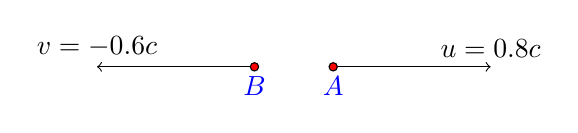
\begin{tikzpicture}
        \draw[->] (3,0,0) -- (5,0,0) node[above]{$u=0.8c$};
        \draw[->] (2,0,0) -- (0,0,0) node[above]{$v=-0.6c$};        
        
        \fill[draw=black,fill=red] (3,0,0) circle[radius=1.5pt] node[below , color = blue]{$A$};
        \fill[draw=black,fill=red] (2,0,0) circle[radius=1.5pt] node[below , color = blue]{$B$};
    \end{tikzpicture}
\end{center}
Consider the frame $S'$ be the rocket B therefore $v =-0.6c$ , so the velocity of the rocket A will be $u = 0.8c$ , we want to find $u'$
\[
\because u = \frac{u'+v}{1+\frac{u'v}{c^2}}    
\]
\[
    0.8c = \frac{u'-0.6c}{1-\frac{(0.6c)u'}{c^2}}    
\]
\[
(0.8c)\left(1-\frac{0.6u'}{c}\right) = u' - 0.6c
\]
\[
    0.8c-(0.8)(0.6)u' = u' - 0.6c
\]
\[
1.4c = (1+.48)u' 
\]
\[
u' =\frac{1.4}{1.48}c = \frac{140}{148}c = 0.94c
\]
\end{example}
\begin{example}
    A rocket is chasing enemy's space-ship an observer on the earth sees the velocity of the rocket 
    $2.5 \times 10^{10}\si{cm/sec}$ and the space-ship $2 \times 10^{10}\si{cm/sec}$ calculate the velocity of enemy's ship as seen by the rocket.
\begin{center}
    ------ \textcolor{Solution}{Solution} ------
\end{center}
Consider the rocket is the frame $S'$ moving with velocity $v=2.5 \times 10^{10}\si{cm/sec}$
and the velocity of the enemy's ship with respect to $S$ is $u=2 \times 10^{10}\si{cm/sec}$ 
we want to find $u'$ of the enemy's ship with respect to the rocket(frame $S'$)
\[
    u = \frac{u'+v}{1+\frac{u'v}{c^2}} 
    \hspace{2cm} 
    c = 3 \times 10^{10}\si{cm/sec}
\]
\[
    2 \times 10^{10} = \frac{u'+2.5 \times 10^{10}}{1+\frac{u'(2.5 \times 10^{10})}{{(3 \times 10^{10})}^2}} 
\]
\[
u' = -\frac{9}{8}\times 10^{10} = -1.125 \times 10^{10}\si{cm/sec^2}
\]
which is a logical answer since the rocket moving with velocity faster than the space ship the rocket will see it move in the opposite direction
\end{example}
\begin{example}
    Show that the velocity $u'$ and $u$ measured in the frames $S'$ and $S$ are related by 
\[
\sqrt{1-\frac{{u'}^2}{c^2}} = \sqrt{\frac{\left(1-\frac{v^2}{c^2}\right)\left(1-\frac{u^2}{c^2}\right)}{{\left(1-\frac{u_x v}{c^2}\right)}^2}}
\]
where $v$ is the velocity of $S'$ relative to S
\begin{center}
    ------ \textcolor{Solution}{Solution} ------
\end{center}
\begin{align*}
    \because {u'}^2         &= {u'_x}^2+{u'_y}^2+{u'_z}^2\\
                            &= {\left(\frac{u_x -v}{1-\frac{u_x v}{c^2}}\right)}^2 + \frac{u_y^2}{\beta^2{\left(1-\frac{u_x v}{c^2}\right)}^2} + \frac{u_z^2}{\beta^2{\left(1-\frac{u_x v}{c^2}\right)}^2}\\
                            &= \frac{1}{{\left(1-\frac{u_x v}{c^2}\right)}^2} \left[ {(u_x - v)}^2 + \left(u_y^2 + u_z^2\right)\left(1-\frac{v^2}{c^2}\right)  \right] \ \ \ \ \ \ \ \ \times\frac{-1}{c^2} + 1\\
1-\frac{{u'}^2}{c^2}        &= 1 - \frac{1}{c^2{\left(1-\frac{u_x v}{c^2}\right)}^2} \left[ {(u_x - v)}^2 + \left(u_y^2 + u_z^2\right)\left(1-\frac{v^2}{c^2}\right)  \right]\\
                            &= \frac{1}{{\left(1-\frac{u_x v}{c^2}\right)}^2} \left[ {\left(1-\frac{u_x v}{c^2}\right)}^2 - \frac{u_x^2}{c^2} - \frac{v^2}{c^2} + 2\frac{u_x v}{c^2} - \frac{u_y^2}{c^2} - \frac{u_z^2}{c^2} + \frac{u_y^2 v^2}{c^4} + \frac{u_z^2 v^2}{c^4}\right]\\
                            &= \frac{1}{{\left(1-\frac{u_x v}{c^2}\right)}^2} \left[ 1 -2\frac{u_x v}{c^2} + \frac{u_x^2 v^2}{c^4} - \frac{u_x^2}{c^2} - \frac{v^2}{c^2} + 2\frac{u_x v}{c^2} - \frac{u_y^2}{c^2} - \frac{u_z^2}{c^2} + \frac{u_y^2 v^2}{c^4} + \frac{u_z^2 v^2}{c^4}\right]\\
                            &= \frac{1}{{\left(1-\frac{u_x v}{c^2}\right)}^2} \left[ 1 -\left(\frac{u_x^2}{c^2} + \frac{u_y^2}{c^2} + \frac{u_z^2}{c^2}\right) - \frac{v^2}{c^2} +\left(\frac{u_x^2 v^2}{c^4} + \frac{u_y^2 v^2}{c^4} + \frac{u_z^2 v^2}{c^4}\right)\right]\\
                            &= \frac{1}{{\left(1-\frac{u_x v}{c^2}\right)}^2} \left[ 1 -\frac{u^2}{c^2} - \frac{v^2}{c^2} +\frac{u^2 v^2}{c^4}\right]\\
                            &= \frac{1}{{\left(1-\frac{u_x v}{c^2}\right)}^2} \left( 1 -\frac{u^2}{c^2}\right) \left(1 - \frac{v^2}{c^2}\right) \ \ \ \ \ \ \text{by taking the square root for both sides}\\
\sqrt{1-\frac{{u'}^2}{c^2}} &= \sqrt{\frac{\left( 1 -\frac{u^2}{c^2}\right) \left(1 - \frac{v^2}{c^2}\right)}{{\left(1-\frac{u_x v}{c^2}\right)}^2}}
\end{align*}
\end{example}

\begin{example}
if a photon travels in such a way that it moves in $x'\circ y'$-plane and makes an angle $\phi$ with $x'$-axis
of the system $S'$. prove that $u_x^2+u_y^2 = c^2$ for the system $S$
\begin{center}
    ------ \textcolor{Solution}{Solution} ------
\end{center}
before we begin the solution for that Example we can use the Property of the light that it's velocity is constant i.e. independent on either reference frame or the direction  
then the proof is done \\
but we will proof it from scratch
    \begin{Framesofreference}
        \draw[->] (4,0,0) -- (6,1,0) node[above right]{$u' = c$};
        \draw [-]  (4.5,0) arc (1:26.5:.5);
        \draw (4.8,.2,0) node {$\phi$};
    \end{Framesofreference}
\[
\because u'_x = c \cos(\phi) \ \ , \ \ u'_y = c \sin(\phi)
\]
\[
    {u'_x}^2 + {u'_y}^2 = c^2
\]
let the system $S'$ be moving with velocity $v$ relative to $S$ since we have 
\[
    u_x = \frac{u'_x + v}{\left(1 + \frac{vu'_x}{c^2}\right)}
    \ \ , \ \ 
    u_y = \frac{u'_y}{\beta\left(1 + \frac{vu'_x}{c^2}\right)}
    \ \ , \ \ \text{where}
    \ \ \beta = \frac{1}{\sqrt{1-\frac{v^2}{c^2}}}
\]
\begin{align*}
    \therefore {u_x}^2 + {u_y}^2 &= {\left(\frac{c \cos(\phi) -v}{1-\frac{v c\cos(\phi)}{c^2}}\right)}^2 + {\left(\frac{c \sin(\phi)}{1-\frac{v c\cos(\phi)}{c^2}}\right)}^2 \left(1-\frac{v^2}{c^2}\right)\\
                                 &= \frac{c^2}{{\left(c+ v \cos(\phi)\right)}^2}\left[c^2 \cos(\phi)^2 + v^2 + 2cv\cos(\phi) + sin(\phi)^2 (c^2-v^2) \right]\\
                                 &= \frac{c^2}{{\left(c+ v \cos(\phi)\right)}^2}\left[c^2 + 2cv\cos(\phi) + v^2\cos(\phi)^2\right]\\
                                 &= \frac{c^2}{{\left(c+ v \cos(\phi)\right)}^2}{\left(c+ v \cos(\phi)\right)}^2\\
                                 &= c^2
\end{align*}
\end{example}

\newpage

\section{Relativistic Formula For Composition Of Acceleration}
for same $S$ and $S'$ as mentioned before using L.I.T we have 
\[
x= \beta(x'+vt') 
\ \ , \ \ 
y = y' 
\ \ , \ \ 
z = z' 
\ \ , \ \ 
t =\beta\left(t' + \frac{vx'}{c^2}\right)
\]
and we got the components of velocities
\[
u_x = \frac{u'_x + v}{\left(1 + \frac{vu'_x}{c^2}\right)}
\ \ , \ \ 
u_y = \frac{u'_y}{\beta\left(1 + \frac{vu'_x}{c^2}\right)}
\ \ , \ \ 
u_z = \frac{u'_z}{\beta\left(1 + \frac{vu'_x}{c^2}\right)}
\]
to get the Acceleration we will differentiate the velocities components with respect to the time as following
\begin{align*}
    f_x = \frac{du_x}{dt} = \frac{d}{dt}\left(\frac{u'_x+v}{1+\frac{u'_x v }{c^2}}\right)&= \frac{d}{dt'}\left(\frac{u'_x+v}{1+\frac{u'_x v }{c^2}}\right) \frac{dt'}{dt}\\
                          &= \frac{\left(1+\frac{u'_x v }{c^2}\right)\frac{du'_x}{dt'} - \left(u'_x+v\right)\left(\frac{du'_x}{dt'}\frac{v}{c^2}\right)}{{\left(1 + \frac{u'_x v}{c^2}\right)}^2} \times \frac{1}{\beta\left(1 + \frac{u'_x v}{c^2}\right)}\\
                          &= \frac{\left(1+\frac{u'_x v }{c^2}\right)f'_x - \left(u'_x+v\right)\left(f'_x\frac{v}{c^2}\right)}{\beta{\left(1 + \frac{u'_x v}{c^2}\right)}^3}\\
                          &= \frac{f'_x\left(1+\frac{u'_x v }{c^2} -\frac{u'_x v }{c^2} - \frac{v^2}{c^2}\right)}{\beta{\left(1 + \frac{u'_x v}{c^2}\right)}^3}\\
                          &= \frac{f'_x\left(1- \frac{v^2}{c^2}\right)}{\beta{\left(1 + \frac{u'_x v}{c^2}\right)}^3} = \frac{f'_x\frac{1}{\beta^2}}{\beta{\left(1 + \frac{u'_x v}{c^2}\right)}^3}\\
                      f_x &= \frac{f'_x}{\beta^3{\left(1 + \frac{u'_x v}{c^2}\right)}^3}
\end{align*}
and for other acceleration component
\begin{align*}
    f_y = \frac{du_y}{dt} = \frac{d}{dt}\left(\frac{u'_y}{\beta\left(1+\frac{u'_x v }{c^2}\right)}\right) &= \frac{d}{dt'}\left(\frac{u'_y}{\beta\left(1+\frac{u'_x v }{c^2}\right)}\right)\frac{dt'}{dt}\\
                          &= \frac{\left(1+\frac{u'_x v }{c^2}\right)f'_y - u'_y\frac{v}{c^2}f'_x}{{\beta\left(1 + \frac{u'_x v}{c^2}\right)}^2} \times \frac{1}{\beta\left(1 + \frac{u'_x v}{c^2}\right)}\\
                          &= \frac{\left(1+\frac{u'_x v }{c^2}\right)f'_y - u'_y\frac{v}{c^2}f'_x}{{\beta^2\left(1 + \frac{u'_x v}{c^2}\right)}^3}\\
                      f_y &=\frac{1}{\beta^2} \left[ \frac{f'_y}{{\left(1+\frac{u'_x v }{c^2}\right)}^2} - \frac{u'_y\frac{v}{c^2}f'_x}{{\left(1 + \frac{u'_x v}{c^2}\right)}^3}\right]
\end{align*}
similarly
\[
    f_z = \frac{1}{\beta^2} \left[ \frac{f'_z}{{\left(1+\frac{u'_x v }{c^2}\right)}^2} - \frac{u'_z\frac{v}{c^2}f'_x}{{\left(1 + \frac{u'_x v}{c^2}\right)}^3}\right]
\]
therefore the acceleration components are given as following
\[
f_x = \frac{f'_x}{\beta^3{\left(1 + \frac{u'_x v}{c^2}\right)}^3}
\ \ , \ \ 
f_y =\frac{1}{\beta^2} \left[ \frac{f'_y}{{\left(1+\frac{u'_x v }{c^2}\right)}^2} - \frac{u'_y\frac{v}{c^2}f'_x}{{\left(1 + \frac{u'_x v}{c^2}\right)}^3}\right]
\ \ , \ \ 
f_z = \frac{1}{\beta^2} \left[ \frac{f'_z}{{\left(1+\frac{u'_x v }{c^2}\right)}^2} - \frac{u'_z\frac{v}{c^2}f'_x}{{\left(1 + \frac{u'_x v}{c^2}\right)}^3}\right]
\]
\subsection{Special Case For Acceleration}
consider the case in which a particle under consideration is at rest momentarily relative to $S'$ i.e. 
$
u'_x =0
\ \ , \ \ 
u'_y =0
\ \ , \ \ 
u'_z =0
$
in this condition the acceleration components will be 
\[
f_x =\frac{f'_x}{\beta^3}
\ \ , \ \ 
f_y =\frac{f'_y}{\beta^2}
\ \ , \ \ 
f_z =\frac{f'_z}{\beta^2}
\]
\subsection{Examples}
\begin{example}
a particle instantaneously at rest in frame of reference $S'$ experiences an acceleration in it represented by a vector 
\[
\vec{f'} = 3 \hat{i} + 4\hat{j} + 12\hat{k}
\]
what is the acceleration measured from the frame of reference $S$ given that $S'$ is moving with velocity 0.98c relative to the frame $S$ along the positive direction of $x$-axis
\begin{center}
    ------ \textcolor{Solution}{Solution} ------
\end{center}
\[
    \because \text{ the particle instantaneously at rest }    
\]
\[
\therefore
u'_x =0
\ \ , \ \ 
u'_y =0
\ \ , \ \ 
u'_z =0
\]
\[
\therefore
f_x =\frac{f'_x}{\beta^3}
\ \ , \ \ 
f_y =\frac{f'_y}{\beta^2}
\ \ , \ \ 
f_z =\frac{f'_z}{\beta^2}
\]
\[
\beta = \frac{1}{\sqrt{1-\frac{v^2}{c^2}}} =  \frac{1}{\sqrt{1-\frac{{(0.98c)}^2}{c^2}}} = \frac{1}{\sqrt{1-{(0.98)}^2}} = \frac{1}{\sqrt{0.04}} = \frac{1}{0.2} = 5
\]
\[
\therefore   
f_x =\frac{3}{5^3} =0.024
\ \ , \ \ 
f_y =\frac{4}{5^2} =0.16
\ \ , \ \ 
f_z =\frac{12}{5^2} = 0.48
\]
\[
\therefore \vec{f} = 0.024 \hat{i} + 0.16 \hat{j} + 0.48\hat{k}
\]
\end{example}

\newpage

\section{Relativity Of Mass}
consider two frames $S$ and $S'$ as mentioned before.
let $m_1$ and $m_2$ are the masses of two identical particle $A,B$ when they at rest in $S$ i.e. $m_1=m_2=m_o$ where $m_o$ is the rest mass of the particles moving with velocity $u' , -u'$ in $S'$ approach each other 
\begin{Framesofreference}
    \draw[->] (5.5,1,0) -- (5.9,1,0) node[above]{$u'$};
        \fill[draw=black,fill=red] (5.5,1,0) circle[radius=2pt];
        \draw (5.5,.9,0) node[below] {$m_1$};
        \draw (5.5,1,0) node[left , blue] {$A$};

        \draw[->] (7,1,0) -- (6.6,1,0) node[above]{$-u'$};
        \fill[draw=black,fill=red] (7,1,0) circle[radius=2pt];
        \draw (7,.9,0) node[below] {$m_2$};
        \draw (7,1,0) node[right,blue] {$B$};
\end{Framesofreference}
the velocity of the two particles in $S$ are given by the Relativistic addition of velocities as 
\[
    u_1 = \frac{u' + v}{1 + \frac{vu'}{c^2}}
    \ \ , \ \ 
    u_2 = \frac{-u' + v}{1 - \frac{vu'}{c^2}}
\]
at the instant of collision the two particle are momentarily at rest with respect to $S'$ but as seen by observer in $S$ they are moving with velocity $v$
\\by using the conservation of momentum 
\begin{align*}
    m_1 u_1 + m_2 u_2 &= (m_1+m_2)v\\
    m_1 \left(\frac{u' + v}{1 + \frac{vu'}{c^2}}\right) + m_2 \left(\frac{- u' + v}{1 - \frac{vu'}{c^2}}\right) &=(m_1+m_2)v\\
    m_1 \left(\frac{u' + v}{1 + \frac{vu'}{c^2}} - v\right) &= m_2 \left(v - \frac{- u' + v}{1 - \frac{vu'}{c^2}}\right)\\
    m_1 \left(\frac{u' - \frac{u'v^2}{c^2}}{1 + \frac{vu'}{c^2}}\right) &= m_2 \left(\frac{u' - \frac{u'v^2}{c^2}}{1 - \frac{vu'}{c^2}}\right)\\
    \frac{m_1}{1 + \frac{vu'}{c^2}}&= \frac{m_2}{1 - \frac{vu'}{c^2}}\\
    \frac{m_1}{m_2}&= \frac{1 + \frac{vu'}{c^2}}{1 - \frac{vu'}{c^2}}  \ \ \ \ \Longrightarrow  \circled{1}
\end{align*}
\begin{align*}
    \because u_1^2 &= {\left(\frac{u' + v}{1 + \frac{vu'}{c^2}}\right)}^2\\
            1-\frac{u_1^2}{c^2} &=1 - \frac{1}{c^2}{\left(\frac{u' + v}{1 + \frac{vu'}{c^2}}\right)}^2\\
                                &=\frac{{\left(1 + \frac{vu'}{c^2}\right)}^2 - {\left(\frac{u'+v}{c}\right)}^2}{{\left(1 + \frac{vu'}{c^2}\right)}^2}\\
    \sqrt{1-\frac{{u'_1}^2}{c^2}} &= \sqrt{\frac{\left( 1 -\frac{{u'}^2}{c^2}\right) \left(1 - \frac{v^2}{c^2}\right)}{{\left(1+\frac{u' v}{c^2}\right)}^2}}\\
    1+\frac{u' v}{c^2}&= \sqrt{\frac{\left( 1 -\frac{{u'}^2}{c^2}\right) \left(1 - \frac{v^2}{c^2}\right)}{1-\frac{{u'_1}^2}{c^2}}}
\end{align*}
similarly
\[
    1-\frac{u' v}{c^2} = \sqrt{\frac{\left( 1 -\frac{{u'}^2}{c^2}\right) \left(1 - \frac{v^2}{c^2}\right)}{1-\frac{{u'_2}^2}{c^2}}}    
\]
substitute those in equation \circled{1}
\[
    \frac{m_1}{m_2} = \sqrt{\frac{1 - \frac{u^2_2}{c^2}}{1 - \frac{u^2_1}{c^2}}}    
\]
now if the particle $B$ is moving with zero velocity in frame $S$ before collision i.e.
we have $u_2=0$ and $m_2=m_o$ rest mass of the particle
\[
\therefore  \frac{m_1}{m_o} = \frac{1}{\sqrt{1 - \frac{u^2_1}{c^2}}} 
\]
\[
    m_1 = \frac{m_o}{\sqrt{1 - \frac{u^2_1}{c^2}}} 
\]
since the particles are exactly identical , the rest mass of the other particle is also $m_o$
\[
\therefore \text{ by replacing } m_1 \text{ by } m \text{ and } u_1 \text{ by } u
\]
\[
\therefore     m = \frac{m_o}{\sqrt{1 - \frac{u^2}{c^2}}} 
\]
\begin{observation}
    if $ u \to c \ \ \therefore m \to \infty$ , this means that no material particle can have velocity $\geq$ c
\end{observation}
\begin{observation}
    if $ u \ll c \ \ \therefore \frac{u^2}{c^2} $ can be ignored $ \ \ \therefore m \simeq m_o $\\
    this means that at small velocities (compared to c) the difference between $m$ and $m_o$ is too small to be detectable
\end{observation}
\subsection{Transformation Formula For Mass}
Consider the two frames $S$ and $S'$ , $S'$ is moving with velocity $v$ along $x$-axis with respect to $S$. let $m$ and $m'$ be the mass of a body in $S$ and $S'$ , which is moving with velocity $u$ and $u'$ in $S$ and $S'$ respectively
\[
\therefore     m = \frac{m_o}{\sqrt{1 - \frac{u^2}{c^2}}}  \ \ \ \ \  \text{and} \ \ \ \ \ m' = \frac{m_o}{\sqrt{1 - \frac{{u'}^2}{c^2}}} 
\]
\[
    \frac{m}{m'} = \sqrt{\frac{1 - \frac{{u'}^2}{c^2}}{1 - \frac{u^2}{c^2}}}        
\]
\[
\because 1-\frac{{u'}^2}{c^2} = \frac{\left( 1 -\frac{u^2}{c^2}\right) \left(1 - \frac{v^2}{c^2}\right)}{{\left(1-\frac{u_x v}{c^2}\right)}^2}    
\]
\[
\therefore \frac{\left(1-\frac{{u'}^2}{c^2}\right)}{\left( 1 -\frac{u^2}{c^2}\right)} = \frac{\left(1 - \frac{v^2}{c^2}\right)}{{\left(1-\frac{u_x v}{c^2}\right)}^2}     
\]
\[
\therefore \frac{m}{m'}  =\sqrt{\frac{\left(1 - \frac{v^2}{c^2}\right)}{{\left(1-\frac{u_x v}{c^2}\right)}^2}} = \frac{1}{\beta\left(1-\frac{u_x v}{c^2}\right)}
\]
\[
\therefore m' = m \beta\left(1-\frac{u_x v}{c^2}\right)
\]
this is the transformation formula for mass

\section{Einstein's Mass-Energy Relation}
Consider the two frames $S$ and $S'$ , $S'$ is moving with velocity $v$ along $x$-axis with respect to $S$.
let a particle of mass $m$ be moving with velocity $u$ along $x$-axis in $S$\\
if a force $\vec{F}$ is applied on this particle, the increase in the kinetic energy of the particle is 
\[
dT = \vec{F} \cdot d\vec{r} = \vec{F} \cdot \vec{u} \ dt \ \ \ \ \ \ \Longrightarrow \circled{1}
\]
\[
\because  \vec{F} dt = m \ d\vec{u} + \vec{u} \ dm
\]
\[
\therefore dT = mu \ du + u^2 \ dm    \ \ \ \ \ \ \Longrightarrow \circled{2}
\]
\[
\because m = \frac{m_o}{\sqrt{1 - \frac{u^2}{c^2}}} 
\]
\[
\therefore dm = \frac{m \ u \ du}{c^2 - u^2}
\]
\[
\therefore du = \frac{(c^2 - u^2)}{mu} dm
\]
substitute in \circled{2}
\[
\circled{2}  \Longrightarrow \ \ \ \ \  dT = c^2 \ dm
\]
therefore the total K.E (T) is given by 
\[
\int_{0}^{T} dT = \int_{m_o}^{m} c^2 \ dm
\]
\[
T = m \ c^2 - m_o \ c^2
\]
and because the total Energy (E) is equal to K.E + the rest energy then by adding $m_o c^2$ we get 
\[
E = MC^2
\]
which is the famous Einstein's equation of special relativity
\begin{figure*}[b]
    \begin{enrichment}{Albert Einstein}{Einstein.jpg}{3}{.77}{.2}
        Albert Einstein, the brilliant physicist and mathematician Born in Ulm Germany in 1879,
        His theory of relativity, first published in 1905, transformed our understanding of space, time, and gravity. 
        Einstein's equation, $E=mc^2$, became synonymous with the concept of mass-energy equivalence and had profound implications for nuclear physics.
        His relentless curiosity, creative thinking, and deep insights reshaped the foundations of modern science, making Albert Einstein one of the most influential figures in history.
    \end{enrichment}
\end{figure*}
\subsection{Deductions on Einstein’s Equation}

\textbf{(I)} by using the kinetic Energy formula
\[
\because T = m c^2 - m_o c^2 = \frac{m_o c^2}{\sqrt{1 - \frac{u^2}{c^2}}}  - m_o c^2 = m_o c^2 \left[{\left(1- \frac{u^2}{c^2}\right)}^{-\frac{1}{2}}-1\right]
\]
now if $\frac{u}{c} \ll 1 $ then by using binomial expansion the power $-\frac{1}{2}$ gives infinite terms but after the second term the value of them can be neglected because they are very small  
\[
\therefore T = m_o c^2 \left[{\left(1+ \frac{u^2}{2c^2} + \dots \right)}-1\right] \simeq m_o c^2 \times \frac{u^2}{2c^2} = \frac{1}{2} m_o u^2
\]
which is the formula of the kinetic Energy in the classical mechanics\\

\textbf{(II)} since the kinetic energy is given by
\[
T = m_o c^2 \left[{\left(1- \frac{u^2}{c^2}\right)}^{-\frac{1}{2}}-1\right]
\]
if $u \to c  \ \ \ \  \therefore T \to \infty $ it means that if we want to accelerate a particle up to the speed of light it will take infinite amount of energy
\subsection{Transformation formula for momentum and Energy}
Consider the two frames $S$ and $S'$ , $S'$ is moving with velocity $v$ along $x$-axis with respect to $S$. let $m$ and $m'$ be the mass of a body in $S$ and $S'$ , which is moving with velocity $u$ and $u'$ in $S$ and $S'$ respectively
then we have the relations
\[
u'_x = \frac{u_x - v}{\left(1 - \frac{vu_x}{c^2}\right)}
\ \ , \ \ 
u'_y = \frac{u_y}{\beta\left(1 - \frac{vu_x}{c^2}\right)}
\ \ , \ \ 
u'_z = \frac{u_z}{\beta\left(1 - \frac{vu_x}{c^2}\right)}
\]
\[ 
    m' = m \beta\left(1-\frac{u_x v}{c^2}\right) \ \ \ \ \ \ \ \ \text{ where } \ \ \beta = \frac{1}{\sqrt{1-\frac{v^2}{c^2}}}
\]
the component of the momentum $P$ are 
\[
P_x = m \ u_x
\ \ , \ \    
P_y = m \ u_y
\ \ , \ \  
P_z = m \ u_z
\ \ \ \  
\text{ in the system } S
\]
we need to find the equivalent in the system $S'$
\[
P'_x = m'u'_x = m \beta\left(1-\frac{u_x v}{c^2}\right) \left(\frac{u_x - v}{1 - \frac{vu_x}{c^2}}\right) = \beta\left(m u_x - m v\right)
\]
\[
\therefore     P'_x = \beta\left(P_x - m v\right) = \beta\left(P_x - \frac{Ev}{c^2}\right)  \ \ \ \ \ \ \ \ \ \because E=m c^2
\]
also
\[
P'_y = m'u'_y = m \beta\left(1-\frac{u_x v}{c^2}\right) \frac{u_y}{\beta\left(1 - \frac{vu_x}{c^2}\right)} = m u_y = P_y
\]
\[
P'_z = m'u'_z = m \beta\left(1-\frac{u_x v}{c^2}\right) \frac{u_z}{\beta\left(1 - \frac{vu_x}{c^2}\right)} = m u_z = P_z
\]
now for the Energy
\[
E' = m'\,c^2 = m\,\beta\left(1-\frac{u_x v}{c^2}\right) c^2 = \beta\left(m\,c^2 - m\, u_x\, v\right) = \beta\left(E - P_x\, v\right)
\]
therefore we have the following
\[
    P'_x = \beta\left(P_x - \frac{Ev}{c^2}\right)
    \ \ , \ \  
    P'_y = P_y
    \ \ , \ \  
    P'_z = P_z
    \ \ , \ \ 
    E' =\beta\left(E - P_x\, v\right)
\]
we notice that those transformations are exactly similar to the $x',y',z',t'$ transformations
\subsection{Examples}
\begin{example}
proof that $P^2 - \frac{E^2}{c^2}$ is Lorentz invariant
\begin{center}
    ------ \textcolor{Solution}{Solution} ------
\end{center}
Lorentz invariant means that the formula form will not change when change to other frame i.e. we need to prove that 
\[
    P^2 - \frac{E^2}{c^2} = {P'}^2 - \frac{{E'}^2}{c^2}
\]
\begin{align*}
    {P'}^2 - \frac{{E'}^2}{c^2} &={P'_x}^2 + {P'_y}^2 + {P'_z}^2 - \frac{\beta^2{\left(E - P_x\, v\right)}^2}{c^2}\\
                                &=\beta^2{\left(P_x - \frac{Ev}{c^2}\right)}^2 + {P'_y}^2 + {P'_z}^2 - \frac{\beta^2{\left(E - P_x\, v\right)}^2}{c^2}\\
                                &=\beta^2\left(P_x^2 + \frac{E^2v^2}{c^4} - 2\frac{P_x v E }{c^2} - \frac{E^2}{c^2} - \frac{P_x^2 v^2}{c^2} + 2\frac{P_x v E}{c^2}\right) + {P'_y}^2 + {P'_z}^2\\
                                &=\beta^2\left(P_x^2 + \frac{E^2v^2}{c^4} - \frac{E^2}{c^2} - \frac{P_x^2 v^2}{c^2}\right) + {P'_y}^2 + {P'_z}^2\\
                                &=\beta^2\left(P_x^2\left(1 - \frac{v^2}{c^2}\right)-\frac{E^2}{c^2}\left(1 - \frac{v^2}{c^2}\right)\right) + {P'_y}^2 + {P'_z}^2\\
                                &=\beta^2\left(\left(P_x^2 - \frac{E^2}{c^2} \right)\left(1 - \frac{v^2}{c^2}\right)\right) + {P'_y}^2 + {P'_z}^2\\
                                &=\beta^2\left(\left(P_x^2 - \frac{E^2}{c^2}\right)\frac{1}{\beta^2}\right) + {P'_y}^2 + {P'_z}^2\\
                                &=P_x^2 - \frac{E^2}{c^2} + {P'_y}^2 + {P'_z}^2 = P^2 - \frac{E^2}{c^2}
\end{align*}
\end{example}
\begin{example}
proof that $x^2 +y^2+z^2-c^2t^2$ is Lorentz invariant
\begin{center}
    ------ \textcolor{Solution}{Solution} ------
\end{center}
\begin{align*}
    {x'}^2 +{y'}^2+{z'}^2-c^2{t'}^2 &= \beta^2{(x-vt)}^2 + y^2 + z^2 - c^2\beta^2{\left(t - \frac{vx}{c^2}\right)}^2\\ 
                                    &= \beta^2\left[x^2 + v^2t^2 - 2xvt - c^2t^2 - \frac{v^2x^2}{c^2} + 2xvt\right] + y^2 + z^2\\ 
                                    &= \beta^2\left[\left(x^2 - c^2t^2\right) \left(1 - \frac{v^2}{c^2}\right)\right] + y^2 + z^2 = x^2 +y^2+z^2-c^2t^2
\end{align*}
\begin{figure*}[b]
    \begin{enrichment*}{Spacetime Interval}
        the relation $\mathbf{x^2 +y^2+z^2-c^2t^2}$ is known as the spacetime interval in the context of special relativity.
        It represents the distance between two events in a four-dimensional spacetime,
        where x, y, and z represent the spatial coordinates, t represents the time coordinate
        The minus sign with the time component is a consequence of the geometry of spacetime and the signature convention used in special relativity.
        the spacetime interval is defined using a metric with a signature convention of $(-, +, +, +)$, which means that the time component has an opposite sign compared to the spatial components.
    \end{enrichment*}
    \end{figure*}
\end{example}



\begin{example}
proof that $P^2 - \frac{E^2}{c^2} = -m_o^2 c^2$
\begin{center}
    ------ \textcolor{Solution}{Solution} ------
\end{center}
\begin{align*}
    P^2 - \frac{E^2}{c^2} &= P_x^2 + P_y^2 + P_z^2 - \frac{m^2 c^4}{c^2}\\
                          &= m^2 u_x^2 + m^2 u_y^2 + m^2 u_z^2 - m^2 c^2\\
                          &= m^2 \left(u_x^2 + u_y^2 + u_z^2\right) - m^2 c^2\\
                          &= m^2 u^2 - m^2 c^2 = \frac{m_o^2}{1 - \frac{u^2}{c^2}} (u^2 - c^2) = -m_o^2 c^2
\end{align*}
\end{example}
\begin{example}
calculate the kinetic energy of an electron moving with a velocity of 0.98c
\begin{center}
    ------ \textcolor{Solution}{Solution} ------
\end{center}
\[
\because T = mc^2 - m_o c^2 = m_o c^2 \left[\frac{1}{\sqrt{1- \frac{u^2}{c^2}}}-1\right]
\]
since $u= 0.98c$ and $m_o = 9\times 10^{-28}\si{gm}$
\[
\therefore T = m_o c^2 \left[\frac{1}{\sqrt{1- 0.98^2}}-1\right]  = \frac{0.801}{0.199}m_o c^2 = 3.26 \times 10^{-6} \si{erg}
\]
\end{example}
\begin{example}
what is the increase in the relativistic mass of a particle of rest mass 1gm when it's moving with velocity of 0.8c. hence find it's K.E
\begin{center}
    ------ \textcolor{Solution}{Solution} ------
\end{center}
\[
m_o = 1gm \ \ \ \ \ \ \text{and} \ \ \ \ \ \ m = \frac{m_o}{\sqrt{1 - \frac{u^2}{c^2}}} = \frac{1}{\sqrt{1 - 0.8^2}} = 1.666\si{gm}
\]
\[
\therefore \text{the increase in it's mass } \Delta m = m-m_o = 0.666\si{gm} 
\]
\[
\text{and it's K.E } = (m-m_o)c^2 = (0.666){(3 \times 10^{10})}^2 = 5.994\times 10^{20}\si{erg}
\]
\end{example}

\begin{example}
the rest masses of a proton and a neutron are $1.6725 \times 10^{-24}$ gm and $1.6748 \times 10^{-24}$ gm.
the observed mass of the deutron\footnote{a type of nucleus composed of one proton and one neutron}
is $3.3433 \times 10^{-24}$ gm. calculate the binding energy
\begin{center}
    ------ \textcolor{Solution}{Solution} ------
\end{center}
\begin{align*}
    \Delta m &= (\text{mass of proton + mass of neotron}) - (\text{mass of deutron})\\
             &= (1.6725 + 1.6748)\times 10^{-24} - 3.3433 \times 10^{-24}\\
             &= 0.004 \times 10^{-24} = 4 \times 10^{-27} \text{gm}
\end{align*}
\begin{align*}
    \text{binding energy } &= \Delta E \\
                           &= \Delta m c^2\\
                           &= \left(4 \times 10^{-27}\right)\times{\left(3 \times 10^{10}\right)}^2\\                           
                           &=36\times 10^{-7}\text{erg}
\end{align*}
\end{example}

\begin{example}
calculate the rest mass of a particle whose momentum is $\frac{130}{c}$MeV when it's kinetic energy is $50$MeV
\begin{center}
    ------ \textcolor{Solution}{Solution} ------
\end{center}
\[
    \because P^2 - \frac{E^2}{c^2} = -m_o^2 c^2 \ \ \ \ \ \text{and} \ \ \ \ \ E = T + m_o c^2
\]
\begin{align*}
\therefore {(T + m_o c^2)}^2 &= P^2c^2 + m_o^2 c^4 \\
            T^2 + 2T m_o c^2 &= P^2c^2\\
            m_0 &= \frac{P^2c^2 - T^2}{2T c^2} = \frac{{(130)}^2 - {(50)}^2}{100 c^2}\\
                &= \frac{144}{c^2} \text{MeV} = 2.56 \times 10^{-25}\si{gm}
\end{align*}
\end{example}
\begin{example}
At what velocity does a particle travel if it's kinetic energy is twice it's rest mass energy?
\begin{center}
    ------ \textcolor{Solution}{Solution} ------
\end{center}
\[
E = T + m_o c^2 = 2 m_o c^2 + m_o c^2  = 3 m_o c^2
\]
\begin{align*}
    m c^2 &= 3 m_o c^2\\
    \frac{m_o}{\sqrt{1 - \frac{u^2}{c^2}}}c^2 &= 3 m_o c^2\\
    \frac{1}{\sqrt{1 - \frac{u^2}{c^2}}} &= 3\\
    1 - \frac{u^2}{c^2} &= \frac{1}{9}\\
    u &= 0.943c
\end{align*}
\end{example}
\begin{example}
calculate the momentum of a neutron whose rest mass energy is 940 MeV and K.E is 200 MeV
\begin{center}
    ------ \textcolor{Solution}{Solution} ------
\end{center}
\begin{align*}
    \because E^2 &= P^2c^2 + m_o^2 c^4 \\    
    {(T + m_o c^2)}^2 &= P^2c^2 + m_o^2 c^4 \\
    P^2c^2 &={(940 + 200)}^2 - {(940)}^2 = 416000\\
    Pc &= \sqrt{416000} = 644.9 \si{MeV}\\
    P &=\frac{644.9}{c} \si{MeV}
\end{align*}
\end{example}
\newpage
\begin{example}
a proton has velocity 0.999c in the laboratory frame. find the energy and the momentum as observer in a frame traveling in the same direction with a velocity 0.99 relative to laboratory given that rest mass of proton = $1.6725 \times 10^{-27}$ kg
\begin{center}
    ------ \textcolor{Solution}{Solution} ------
\end{center}
\[
\because u_x = u = 0.999c \ \ , \ \ v = 0.99c \ \ , \ \ m_o = 1.6725 \times 10^{-24} \si{gm}
\]
\[
E = m c^2  = \frac{m_o c^2}{\sqrt{1 - \frac{u^2}{c^2}}} = \frac{m_o c^2}{\sqrt{1 - 0.998}} = \frac{m_o c^2}{0.0447} = 22.37 m_o c^2
\]
\[
P_x = m u_x = \frac{m_o u_x}{\sqrt{1 - \frac{u^2}{c^2}}} = \frac{m_o (0.999c)}{0.0447} = 22.35 m_o c
\]
we now need to find $E'$ and $P'_x$


\begin{align*}
    \because P'_x &= \beta\left(P_x - \frac{Ev}{c^2}\right) \hspace{2cm} \beta = \frac{1}{\sqrt{1-\frac{v^2}{c^2}}} = \frac{1}{\sqrt{1-0.99^2}} = \frac{1}{0.1411}\\
    &= \frac{1}{0.1411}\left(22.35 m_o c - \frac{(0.99c)(22.37 m_o c^2)}{c^2}\right) = \frac{0.2037}{0.1411}m_o c\\
    &= \frac{0.2037}{0.1411} \times \left(1.6725 \times 10^{-24}\right) \times \left(3 \times 10^{10}\right) = 7.24 \times 10^{-14} \si{gm} \cdot \si{cm/sec}
\end{align*}
and
\begin{align*}
    \because E' &= \beta\left(E - P_xv\right)\\
    &=\frac{1}{0.1411} \left(22.37 m_o c^2 - (0.99c)(22.35 m_o c)\right) = 1.725 m_o c^2\\
    &=1.725 \times \left(1.6725 \times 10^{-24}\right) \times \left(9 \times 10^{20}\right) = 25.965 \times 10^{-4} \si{erg}
\end{align*}
\end{example}
\begin{example}
if the momentum of a particle is given to be $m_o c$ find 
\\(i) it's velocity \ \ (ii) it's mass \ \ (iii) it's kinetic energy
\begin{center}
    ------ \textcolor{Solution}{Solution} ------
\end{center}
\begin{align*}
    \because P^2 - \frac{E^2}{c^2} &= -m_o^2 c^2\\
    {(m_o c)}^2 - \frac{E^2}{c^2} &= -m_o^2 c^2\\
    E &= \sqrt{2} m_o c^2\\
    m c^2 &= \sqrt{2} m_o c^2\\
    \text{then it's mass } m &= \sqrt{2} m_o
\end{align*}
\begin{align*}
    \frac{m_o}{\sqrt{1 - \frac{u^2}{c^2}}} &= \sqrt{2} m_o\\
    1 - \frac{u^2}{c^2} &= \frac{1}{2}\\
    \text{it's velocity } u &= \frac{1}{\sqrt{2}} c
\end{align*}
\[
    \text{and it's kinetic energy } T = \sqrt{2} m_o c^2 - m_o c^2 = \left(\sqrt{2} -1\right)m_o c^2
\]
\begin{center}
    ------ \textcolor{Solution}{Other Solution} ------
\end{center}
\begin{align*}
    P = mu &= m_o c\\
    \frac{m_o u}{\sqrt{1 - \frac{u^2}{c^2}}} &= m_o c\\
    \frac{u^2}{1 - \frac{u^2}{c^2}} &= c^2\\
    u^2 &= c^2 - u^2\\
    \text{it's velocity } u &= \frac{1}{\sqrt{2}} c
\end{align*}
\begin{align*}
    \because mu &= m_o c\\
        m \frac{1}{\sqrt{2}} c &= m_0 c\\
        \text{then it's mass } m &= \sqrt{2} m_o
\end{align*}
\[
    \text{and it's kinetic energy } T = \sqrt{2} m_o c^2 - m_o c^2 = \left(\sqrt{2} -1\right)m_o c^2
\]
\end{example}
\section{Transformation of Force}
Consider the two frames $S$ and $S'$ , $S'$ is moving with velocity $v$ along $x$-axis with respect to $S$.
in the frame $S'$ the force on a particle is given by 
\[
\vec{F'}  = \frac{d\vec{P'}}{dt'}
\]
\begin{align*}
    \therefore F'_x &= \frac{dP'_x}{dt'} = \frac{d}{dt'} \beta\left(P_x - \frac{Ev}{c^2}\right)
                = \frac{d}{dt} \beta\left(P_x - \frac{Ev}{c^2}\right) \frac{dt'}{dt}\\
               &=\frac{\left(\frac{dP_x}{dt} - \frac{dE}{dt}\frac{v}{c^2}\right)}{1 - \frac{vu_x}{c^2}} =\frac{\left(F_x - \frac{dE}{dt}\frac{v}{c^2}\right)}{1 - \frac{vu_x}{c^2}}            
\end{align*}
and since
\begin{align*}
    E^2 &= P^2c^2 + m_o^2 c^4 \\
        &= \left(\vec{P}\cdot\vec{P}\right) c^2 + + m_o^2 c^4\\
\therefore 2E \frac{dE}{dt} &=2 c^2 \vec{P} \frac{d\vec{P}}{dt}\\
        m c^2 \frac{dE}{dt} &=c^2 \vec{P} \cdot \vec{F}\\
        \frac{dE}{dt} &= \frac{\vec{P} \cdot \vec{F}}{m} = \vec{u} \cdot \vec{F}
\end{align*}
so 
\[
F'_x = \frac{\left(F_x - \left(\vec{u} \cdot \vec{F}\right)\frac{v}{c^2}\right)}{1 - \frac{vu_x}{c^2}}
\]
the other relations can be similarly obtained
\[
F'_y = \frac{F_y}{\beta\left(1 - \frac{vu_x}{c^2}\right)}
\]
and 
\[
F'_z = \frac{F_z}{\beta\left(1 - \frac{vu_x}{c^2}\right)}
\]
and for the inverse of those relations just put the $v \to -v$
\[
    F_x = \frac{\left(F_x + \left(\vec{u} \cdot \vec{F}\right)\frac{v}{c^2}\right)}{1 + \frac{vu_x}{c^2}}
    \ \ , \ \  
    F_y = \frac{F_y}{\beta\left(1 + \frac{vu_x}{c^2}\right)}   
    \ \ , \ \  
    F_z = \frac{F_z}{\beta\left(1 + \frac{vu_x}{c^2}\right)}
\]
\subsection{Special Case For Force}
if the particle happens to be at rest in the frame $S$ then $\vec{u} = 0$. then the Forces equation going to be as following
\[
    F'_x = F_x
    \ \ , \ \  
    F'_y = \frac{F_y}{\beta}
    \ \ , \ \  
    F'_z = \frac{F_z}{\beta}
\]
\section{Relativistic Lagrange Equations}
we know that the relativistic K.E of a particle of rest mass $m_o$ and moving with velocity $u$ is given by 
\[
    T = mc^2 - m_o c^2 = m_o c^2 \left[{\left(1- \frac{u^2}{c^2}\right)}^{-\frac{1}{2}}-1\right]    
\]
and since the relativistic momentum is given by 
\[
   P_x = m \dot{x} = \frac{m_o}{\sqrt{1 - \frac{u^2}{c^2}}} \dot{x}
\]
then it's clear that $\frac{\partial T}{\partial \dot{x} }$ doesn't give the relativistic momentum $P_x$ therefore we need to define a function $T^*$ such that 
\[
    P_x = \frac{\partial T}{\partial \dot{x}}
\]
similarly for $y$ and $z$ components
\begin{align*}
    \because T^* &= \frac{\partial T}{\partial \dot{x}} d\dot{x} + \frac{\partial T}{\partial \dot{y}} d\dot{y} + \frac{\partial T}{\partial \dot{z}} d\dot{z}\\
    dT^* &= P_x d\dot{x} + P_y d\dot{y} +P_z d\dot{z}\\
    &=\frac{m_o}{\sqrt{1 - \frac{u^2}{c^2}}} \left( \dot{x}d\dot{x} + \dot{y}d\dot{y} + \dot{z}d\dot{z}  \right)\\
 \text{since } u^2 = \dot{x}^2 + \dot{y}^2 + \dot{z}^2 &\Longrightarrow 2u du =2 \left( \dot{x}d\dot{x} + \dot{y}d\dot{y} + \dot{z}d\dot{z}  \right) \\
    &=\frac{m_o u du}{\sqrt{1 - \frac{u^2}{c^2}}} \\
    \int dT^* &= \int \frac{m_o u du}{\sqrt{1 - \frac{u^2}{c^2}}} \\
\therefore T^* &= - m_o c^2\sqrt{1 - \frac{u^2}{c^2}} + C\\
\text{to determine C, we know that when }& u \ll c  \ \ \therefore T* = \text{ordinary k.e} = \frac{1}{2} m_o u^2\\
\therefore C &= \frac{1}{2} m_o u^2 + m_o c^2 \left(1- \frac{1}{2}\frac{u^2}{c^2}\right)\\
             &= m_o c^2
\end{align*}
\[
\therefore T^* = m_o c^2\left(1- \sqrt{1 - \frac{u^2}{c^2}}\right)
\]
the relativistic Lagrangian L can now be defined as 
\[
L = T^* - V = m_o c^2\left(1- \sqrt{1 - \frac{u^2}{c^2}}\right) - V
\]
now the $\because$ Lagrangian equations are
\[
\frac{d}{dt}\left( \frac{\partial L}{\partial \dot{q_r}} \right) = \frac{\partial L}{\partial q_r}
\]
\[
    \dot{q_r} \equiv  \dot{x} , \dot{y}  , \dot{z}
    \ \ , \ \ 
    q_r \equiv x , y , z
\]
\[
\because \frac{\partial L}{\partial \dot{x}} = \frac{\partial T}{\partial \dot{x}} - 0 = \frac{m_o \dot{x}}{\sqrt{1 - \frac{u^2}{c^2}}}
\ \ \text{ and } \ \ \frac{\partial L}{\partial x} = -\frac{\partial V}{\partial x}
\]
hence the  Lagranges equations becomes
\begin{align*}
    \frac{d}{dt} \left(\frac{m_o \dot{x}}{\sqrt{1 - \frac{u^2}{c^2}}}\right) &= -\frac{\partial V}{\partial x}\\
    \frac{d}{dt} \left(\frac{m_o \dot{y}}{\sqrt{1 - \frac{u^2}{c^2}}}\right) &= -\frac{\partial V}{\partial y}\\
    \frac{d}{dt} \left(\frac{m_o \dot{z}}{\sqrt{1 - \frac{u^2}{c^2}}}\right) &= -\frac{\partial V}{\partial z}
\end{align*}
\begin{figure*}[b]
\begin{enrichment}{Joseph Louis Lagrange}{Lagrange.jpg}{3}{.77}{.2}
    Lagrange was an influential mathematician and physicist of the 18th century. He was born on January 25, 1736, in Turin, Italy, and he made significant contributions to various branches of mathematics, mechanics, and celestial mechanics.
    One of Lagrange's most well-known contributions is his formulation of analytical mechanics, which is now known as Lagrangian mechanics. This groundbreaking approach revolutionized classical mechanics, providing a powerful and elegant method to describe the motion of particles and systems using energy principles and differential equations. His work laid the foundation for later developments in the study of celestial mechanics, making significant contributions to our understanding of the solar system and the motion of celestial bodies.
\end{enrichment}
\end{figure*}

\subsection{The Relativistic Hamiltonian}
we now define the relativistic Hamiltonian as 
\begin{align*}
    H &= \sum P_r\dot{q_r}  - L\\
      &= P_x\dot{x} + P_y\dot{y} + P_z\dot{z} - L\\
      &= \frac{\partial T}{\partial \dot{x}}\dot{x} + \frac{\partial T}{\partial \dot{y}}\dot{y} + \frac{\partial T}{\partial \dot{z}}\dot{z} -L\\
      &= \frac{m_o \dot{x}}{\sqrt{1 - \frac{u^2}{c^2}}}\dot{x} + \frac{m_o \dot{y}}{\sqrt{1 - \frac{u^2}{c^2}}}\dot{y} + \frac{m_o \dot{z}}{\sqrt{1 - \frac{u^2}{c^2}}}\dot{z} -L \\
      &= \frac{m_o}{\sqrt{1 - \frac{u^2}{c^2}}} \left(\dot{x}^2 + \dot{y}^2 + \dot{z}^2\right) - L\\
      &= \frac{m_o u^2}{\sqrt{1 - \frac{u^2}{c^2}}} - m_o c^2\left(1- \sqrt{1 - \frac{u^2}{c^2}}\right) + V\\
      &= \frac{m_o u^2}{\sqrt{1 - \frac{u^2}{c^2}}} + m_o c^2 \sqrt{1 - \frac{u^2}{c^2}} - m_o c^2  + V\\
      &= \frac{m_o}{\sqrt{1 - \frac{u^2}{c^2}}}\left(u^2 + c^2 - u^2\right) - m_o c^2  + V\\
      &= m c^2 - m_o c^2  + V = T + V
\end{align*}
so H represent the total energy \\
to express H in terms of momentum
\begin{align*}
    H &= m c^2 - m_o c^2  + V \\  
    \because E^2 &= P^2c^2 + m_o^2 c^4 \\
    m^2 c^4 &= P^2c^2 + m_o^2 c^4 \\
    \therefore H &= \sqrt{P^2c^2 + m_o^2 c^4} - m_o c^2  + V\\
    &= c\sqrt{P^2 + m_o^2 c^2} - m_o c^2  + V
\end{align*}
This is the relativistic Hamiltonian\\
the relativistic Hamiltonian's canonical equations are 
\begin{figure*}[b]
\begin{enrichment}{William Rowan Hamilton}{Hamilton.png}{2.2}{.82}{.15}
    born on August 4, 1805, in Dublin, Ireland William Rowan Hamilton was an Irish mathematician, physicist, and astronomer who made significant contributions to various fields of science.
    One of Hamilton's most significant achievements was his work on quaternion algebra, which he developed in 1843. Quaternions are a four-dimensional extension of complex numbers, and they played a crucial role in advancing mathematical and physical theories, especially in the study of rotations in three-dimensional space.
\end{enrichment}
\end{figure*}
\[
\dot{x} = \frac{\partial H}{\partial P_x}
\ \ , \ \
\dot{y} = \frac{\partial H}{\partial P_y}
\ \ , \ \
\dot{z} = \frac{\partial H}{\partial P_z}
\ \ \ \
\Longrightarrow  \circled{1}
\]
\[
\dot{P_x} =-\frac{\partial H}{\partial x}
\ \ , \ \
\dot{P_y} =-\frac{\partial H}{\partial y}
\ \ , \ \
\dot{P_z} =-\frac{\partial H}{\partial z}
\ \ \ \
\Longrightarrow  \circled{2}
\]
\[
\text{from }  \circled{1} \Longrightarrow 
\ \ \ \
\dot{x} = \frac{c P_x}{\sqrt{P^2 + m_o^2 c^2}}
\ \ , \ \
\dot{y} = \frac{c P_y}{\sqrt{P^2 + m_o^2 c^2}}
\ \ , \ \
\dot{z} = \frac{c P_z}{\sqrt{P^2 + m_o^2 c^2}}
\]
\[
\because
P_x = \frac{m_o \dot{x}}{\sqrt{1 - \frac{u^2}{c^2}}}
\ \ , \ \
P_y = \frac{m_o \dot{y}}{\sqrt{1 - \frac{u^2}{c^2}}}
\ \ , \ \
P_z = \frac{m_o \dot{z}}{\sqrt{1 - \frac{u^2}{c^2}}}
\]
\begin{align*}
    \text{then from }  \circled{2} \Longrightarrow 
    \ \ \ \
    \frac{d}{dt}\left(\frac{m_o \dot{x}}{\sqrt{1 - \frac{u^2}{c^2}}}\right) &= -\frac{\partial H}{\partial x} = -\frac{\partial V}{\partial x}\\
    \frac{d}{dt}\left(\frac{m_o \dot{y}}{\sqrt{1 - \frac{u^2}{c^2}}}\right) &= -\frac{\partial H}{\partial y} = -\frac{\partial V}{\partial y}\\
    \frac{d}{dt}\left(\frac{m_o \dot{z}}{\sqrt{1 - \frac{u^2}{c^2}}}\right) &= -\frac{\partial H}{\partial z} = -\frac{\partial V}{\partial z}
\end{align*}
\section{Units}
we will consider two systems of units C.G.S (cm , gm , second) and M.K.S (meter , kilogram , second)\\
note the Joule is in M.K.S while the erg in C.G.S
\\\textbf{(I)} in the formula $E = m c^2$ , units of m , c and E are gm , cm/sec , erg.
\\\textbf{(II)} 1eV = one electron volt = $1.6 \times 10^{-12}$ erg
\\\textbf{(III)} 1 Joule = $10^{7}$ erg
\\\textbf{(IV)} 1 MeV = $10^{6}$ eV = $1.6 \times 10^{-6}$ erg
\\\textbf{(V)} rest mass of proton = $1.6725 \times 10^{-24}$ gram
\\\textbf{(VI)} rest mass of neutron = $1.6748 \times 10^{-24}$ gram
\\\textbf{(VII)} rest mass of electron = $9 \times 10^{-28}$ gram
\\\textbf{(VIII)} 1gm = $6 \times 10^{23}$ a.m.u \ \ \ \ (a.m.u = atomic mass unit)
\\\textbf{(IX)} 1 Calory = $4.2 \times 10^7$ erg = 4.2 Joule
\\\textbf{(X)} 1 BeV = $10^{9}$ eV = $1.6 \times 10^{-3}$ erg

\section{What Next}
after finishing this course if you want to continue studying the Special Relativity 
i recommend to you 
\\
\\\textbf{1-} "Special Relativity: A Comprehensive Introduction" by Wolfgang Rindler
\\\textbf{2-} "Spacetime Physics" by Edwin F. Taylor and John Archibald Wheeler
\\\textbf{3-} "Introduction to Special Relativity" by Robert Resnick
\\\textbf{4-} "Special Relativity and Classical Field Theory: The Theoretical Minimum" by Leonard Susskind and Art Friedman
\\\textbf{5-} "Special Relativity: For the Enthusiastic Beginner" by David J. Morin
\\\textbf{6-} "Special Relativity: From Einstein to Strings" by Patricia M. Schwarz and John H. Schwarz
\\\textbf{7-} "Special Relativity in General Frames: From Particles to Astrophysics" by Éric Gourgoulhon
\\\textbf{8-} "Introduction to Special Relativity" by Wolfgang Rindler
\\\textbf{9-} "The Geometry of Special Relativity" by Tevian Dray
\\\\
These books cover a range of topics and levels of difficulty, from introductory to more advanced. You can choose the one that suits your needs and level of understanding.
\\\\
and if you not a fan of books you can check those documentaries
\\
\\\textbf{1-} "The Fabric of the Cosmos" - Hosted by physicist Brian Greene, this four-part series explores fundamental questions about space, time, and the nature of reality, including a segment on Special Relativity.
\\\textbf{2-} "Inside Einstein's Mind" - This documentary takes a closer look at the life and work of Albert Einstein, including his development of the theory of Special Relativity.
\\\textbf{3-} "Light Falls: Space, Time, and an Obsession of Einstein" - This film combines interviews, historical footage, and animation to explore the story of Albert Einstein and his groundbreaking theories, including Special Relativity.
\end{document}